\chapter{Sterile Neutrino Oscillation Inputs Within SBN}
\label{chap:osc_inputs}

In order to perform an oscillation analysis, a number of inputs and analysis choices are required. Typically this involves generating some event sample in each detector for a given analysis, applying a physics hypothesis and some set of systematic uncertainties. A fit comparing the observed and predicted event rate is then performed giving the confidence level of the applied physics hypothesis. This is summarised in \FigureRef{fig:analysis_paradigm} which shows the generic overview of the procedure coupled with the different components. Many of these items are common to all oscillation analyses and are agnostic to the fitting framework. The remainder of this chapter highlights some of the key inputs to the oscillation analysis along with some of the decisions that were made. The actual analysis results are detailed in \SectionRef{chap:VALOR} in addition to explaining how the VALOR framework processes or consumes these inputs where appropriate.

\begin{figure}[!h]
    \centering
    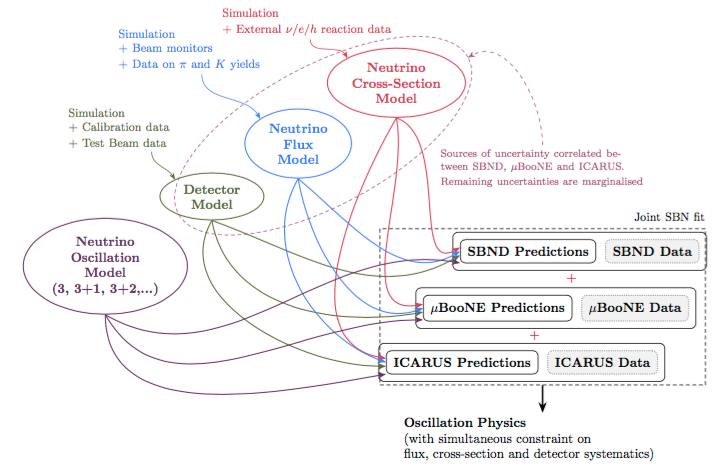
\includegraphics[width = \textwidth]{figures-chap5/valor_analysis.png}
    \caption[SBN Oscillation analysis paradigm.]{Overview of the SBN oscillation analysis paradigm. A given model for the neutrino oscillation, detector, neutrino flux and neutrino cross-section are combined with the appropriate data to give the prediction for the respective detector. Individual detector predictions may be combined to give an overall \gls{sbn} prediction. }
    \label{fig:analysis_paradigm}
\end{figure}

\section{Monte Carlo Event Production}

The events used in this oscillation analysis are truth based with a \textit{pseudo reconstruction} applied. Work on the reconstruction is still in progress and at the time of writing has not been sufficiently completed for it to be possible to generate a fully reconstructed event sample. The pseudo reconstruction involves applying energy smearing and a series of cuts to try and emulate a fully reconstructed sample. The details of the cuts and smearing that were applied to each of the analyses are discussed in \SectionRef{sec:event_selection}.

Both the events for the \numu and \nue sample were generated using \gls{genie}v3 (specifically the G18\_10a\_02\_11a tune) and then propagated through \gls{geant4} using the \gls{larsoft} framework \cite{GENIE}\cite{GENIE_V3_Paper}\cite{GENIE_tune}\cite{Geant4_website}\cite{larsoft}. For the \numu sample, this involved generating $\sim$1,000,000 intrinsic \numu events in each detector. The \nue sample is a little more involved since in addition to generating an intrinsic sample, an oscillated $\numu \rightarrow \nue$ sample, a dirt sample and a cosmic sample also needed to be produced. The oscillated sample is used to mimic the $\nue$ appearance signal whereas the dirt and cosmic samples are backgrounds. The other major background associated with a $\nue$ analysis involves $\numu$. A dedicated sample was not produced to emulate this, but instead, the events from the $\numu$ production were also run through the $\nue$ selection. Table \ref{T:nue_production} outlines the number of events produced for the \nue sample for each sub-sample for each detector. Additionally, the number of events that were selected from each sample are shown for all three detectors. The dirt events were produced with an additional filter at the generation stage which discarded any events where a shower above 10 MeV in the active volume was not present. This filter was used in order to remove any delta rays. Only about 1\% of dirt events would pass this filter so the number of dirt events used in the $\nue$ selection was $\sim$100,000. 


\begin{table}[h!]
\begin{tabular}{c rrrr}
\multirow{2}{*}{Sample} & \multirow{2}{*}{Produced} & \multicolumn{3}{c}{Selected} \\ & & \gls{sbnd} & \gls{microboone} & \gls{icarus}  \\ \hline

Intrinsic $\nue$ & $\sim$1,000,000    & ~$\sim 150,000$ & ~$\sim 140,000$ & ~$\sim 130,000$ \\
Oscillated $\nu$ & $\sim$1,000,000    & ~$\sim 180,000$ & ~$\sim 150,000$ & ~$\sim 140,000$ \\
$\numu$          & {Used \numu sample}& ~$\sim 2,000$ & ~$\sim 3,000$ & ~$\sim 3,000$ \\
Dirt             & $\sim$10,000,000 & $\sim 80$ & ~$\sim 100$ & ~$\sim 300$ \\
Cosmic           & $\sim$100,000    & ~$\sim 1$ & ~$0$ & ~$\sim 30$             

\end{tabular}
\caption[Events generated and selected as part of the \nue sample.]{The number of events produced and selected for each sub-sample of the \nue analysis. The same number of events were produced in each of the three \gls{sbn} detectors.}
\end{table}\label{T:nue_production}

The actual number of real \numu events expected in \gls{sbnd} is well over 5 million for about 3 years of data taking \cite{sbnd_pot}. Generating this many events is not feasible as part of a \gls{mc} production, hence the above number of events were generated. The \gls{mc} events produced have an associated \gls{pot} so the number of events may be scaled to the nominal \gls{pot} of each experiment. For \gls{sbnd} and \gls{icarus} the nominal \gls{pot} is $6.6 \times 10^{20}$ which corresponds to around 3 years of data taking.  Since \gls{microboone} has already been collecting data for some time, the nominal \gls{pot} is $1.32 \times 10^{21}$. Due to scaling the generated event rate to the nominal \gls{pot} this results in non-integer number of events. %as is seen for example in \TableRef{table:sbnd_nue_event_rate}.

\section{Event Reconstruction}

To emulate reconstructed energies, the true energy of particles are smeared. For the \numu sample the following conditions are applied. Primary tracks (which is the leading muon in the final state) contained in the active volume, have their true energy smeared by scaling the energy with a Gaussian which has a standard deviation of 0.02. If the primary track is not contained, the energy is instead smeared by a Gaussian with a standard deviation that is given by $-A\lnOfbraces{BL}$,
where \textit{L} is the track length and $A = 0.102$ and $B = 0.000612$ cm$^{-1}$ \cite{SBN_Proposal}. This emulates the multiple scatterings of the track, but in order for the track to have sufficient resolution, a minimum track length of 100 cm is required. Parameters \textit{A} and \textit{B} were chosen based on the work of \cite{ICARUS_muon_smearing}. Non-primary tracks with a true energy of less than 21 MeV are removed (21 MeV is the kinetic energy threshold for reconstructing tracks \cite{SBN_Proposal}) and any remaining tracks are smeared with a Gaussian which has a standard deviation of 0.05 \cite{SBN_Proposal}. An additional condition that the minimum smeared energy is 0 MeV is applied which ensures that negative energies do not occur.

The values used to determine the degree of energy smearing for the \nue sample are different to the \numu sample. The energy of electron and photon showers are smeared with a Gaussian that has a standard deviation of $0.15/\sqrt{E_{true}}$. Contained muons are smeared with a Gaussian that has a standard deviation of 0.15 whereas the smearing of non-contained muons is not considered. Finally, the hadrons are smeared with a Gaussian that has a standard deviation of 0.05. The same condition ensuring that negative energies are not allowed is again applied. A check is also performed to see if there is more than 50 MeV of hadronic activity at the vertex, which is the threshold for the vertex to be considered visible \cite{SBN_Proposal}. Additionally, the reconstruction is assumed to only be sufficiently accurate for showers above 200 MeV, therefore any events with showers that do not exceed this energy threshold are removed. 

When reconstructed quantities are considered, background events may mimic the key signature of signal events, resulting in events being misidentified. Some of the most common backgrounds to a \gls{cc} inclusive sample in \gls{sbn} will be due to: 

\begin{itemize}
    \item \numu sample: Charged pions which may be produced by \gls{nc} interactions will result in a track that can resemble a muon. Most of the tracks produced by pions will be relatively short at less than 50 cm. 
    
    \item \nue sample: Final state neutral pions which are a result of \gls{nc} interactions decay into two photon showers. 
    \item \nue sample: If the track length is short (< 1 m) and has a single associated \gls{em} shower, \numu \gls{cc} events with a $\mu + \gamma$ in the final state may be mistaken for \nue \gls{cc} events with a $\pi + e$ in the final state.
    \item \nue sample: Cosmic photons may produce electrons in the \gls{tpc} via pair production or Compton scattering. The cosmic photons may be produced in the atmospheric shower or by cosmic muons passing through the detector \cite{SBN_Proposal}. 
\end{itemize}

\section{Event Selection}\label{sec:event_selection}

%The event selections are performed in order to first identify \numu or \nue-like interactions. The selection steps are designed to try and produce a pure $\nu_{\mu, e}$ \gls{cc} inclusive sample for each of the analyses, the details of which are outlined below and are performed for each associated event. 

The event selections are performed in order to first identify \numu or \nue-like interactions which form a \numu or \nue \gls{cc} inclusive sample. The selection steps are designed to produce as pure as possible \gls{cc} inclusive sample by rejecting contributions from other samples such as \gls{nc} or cosmics, the details of which are outlined below. 

\subsection{\texorpdfstring{\numu Selection}{numu Selection}}\label{sec:numu_selection}

 The selection criteria for the \numu sample are as follows:

\begin{enumerate}
  \item Remove any events whose interaction vertex is not located in the fiducial volume. The fiducial volume used is outlined in \TableRef{table:active_and_fiducial_volumes}.
  \item If no muon or charged pion track are produced, remove the event. %A muon corresponds to a \gls{cc} signal event whereas a charged pion is possibly due to \gls{nc} background events. 
  %\item If the primary track has a true kinetic energy less than 21 MeV, remove the event.
  \item If the primary track has a length less than 50 cm and is fully contained in the detector, remove the event.
  \item If the primary track exits the detector and has a length less than 100 cm, remove the event. %For muons exiting the active volume, the energy is estimated via multiple scatterings of the track and in order to measure the multiple scattering with sufficient resolution a minimum track length of a 100 cm is required.
 \item A weight of 0.8 is applied to all selected events to account for an assumed 80\% reconstruction efficiency \cite{SBN_Proposal}. 
\end{enumerate}

\subsection{\texorpdfstring{\nue Selection}{nue Selection}}\label{sec:nue_selection}

The $\nue$ selection follows a similar basis to the $\numu$ selection described in section \ref{sec:numu_selection}, however different criteria for the selection were applied to beam induced TPC events, dirt events and cosmic events, each of which are outlined below. 

\subsubsection*{Beam induced active volume events}

\begin{enumerate}
  \item Remove any events whose interaction vertex is not located in the fiducial volume. The fiducial volume used is outlined in \TableRef{table:active_and_fiducial_volumes}.
  \item If more than one shower arising from the vertex has an energy above a 100 MeV, the event is removed. %Showers arising from the vertex are identified and the reconstructed energy is found from smearing the ionisation deposition. If more than one shower with energy above 100 MeV exists, the event is removed. This removes neutral pion events where the pion decays into two photon showers. 
  \item If there is only one photon candidate in the event, a conversion gap cut is applied rejecting any event where the photon shower occurs more than 3 cm from the vertex. 
  \item A weight of 0.06 is applied to the remaining photons which undergo a dE/dx cut resulting in a 94\% background rejection.
  \item If a misidentified photon originates from a resonant $\numu$ CC interaction, the muon lepton is identified. Events where a muon travels greater than 1 m are assumed to be from $\numu$ CC interactions and the event is removed. 
  %\item Events where the shower has an energy less than 200 MeV are removed.
  \item A weight of 0.8 is applied to all selected events
to account for an assumed 80\% reconstruction efficiency \cite{Dom's_thesis}.
\end{enumerate}

\subsubsection*{Dirt Events}
The selection procedure for dirt events is similar to that of beam induced events outlined above. However, since the vertex for dirt events occurs outside the detector volume, the conversion gap and muon track length cuts are not undertaken \cite{Dom's_thesis}.

\subsubsection*{Cosmic Events}
A largely separate analysis is applied for cosmic events which is as follows:
\begin{enumerate}
    \item  If a cosmic photon initially interacts outside the fiducial volume the event is removed.
    \item Cosmic events which occur outside the beam spill time window are removed if there is no other activity in the TPC during the beam spill time.
    \item 95\% of cosmic events occurring within the beam spill window are removed by use of the PDS and CRT systems and taking advantage of the bucket structure of the beam.
    \item Same dE/dx cut as described above. 
    %\item Events below a reconstructed energy of 200 MeV are removed.
    \item A topological cosmic cylinder cut is applied to cosmic photons which originate from cosmic muons that pass through the TPC. These can be removed by a fiducial volume cut corresponding to a cylinder of radius 15 cm around the cosmic muon \cite{Dom's_thesis}. 
\end{enumerate}

\section{Reaction Modes}
The reaction modes define the topology of neutrino interactions. Categorising neutrino events is a requirement for handling systematic uncertainties since these are reaction mode dependent. The reaction modes are grouped into two sets: the \textit{fine} reaction modes which outline the complete list of all possible reaction modes and the \textit{coarse} reaction modes which define a broader class of interaction which encompass one or more fine reaction mode. The fine reaction modes are listed in \TableRef{table:fine_reac_modes} and are typically used at the analysis level. The coarse reaction modes used depend on the analysis channel and are listed in \TableRef{table:coarse_reac_modes}. They are usually only used when displaying data such as in a breakdown of event rate spectra since using the complete list of reaction modes would be impractical. 

% Fine reaction modes
\begin{table}[t!]
  \renewcommand{\arraystretch}{1.6}
  \begin{tabular}{>{\centering\arraybackslash}m{4cm} 
                  >{\centering\arraybackslash}m{4cm}
                  >{\centering\arraybackslash}m{4cm}}
  
    \toprule
    \multicolumn{3}{c}{\textit{Fine Reaction Modes}} \\
    $\numu$, $\numubar$ & $\nue$, $\nuebar$ & $\numu \rightarrow \nue, \numubar \rightarrow \nuebar$ \\
    \midrule
    CC QE 0\pi                     & CC QE 0\pi                    & CC QE 0\pi \\
    NC~Elastic                 & NC~Elastic                & CC 2p2h\\ 
    CC, NC 2p2h                 & CC, NC 2p2h                & CC 1$\pi^{\pm}$ \\  
    CC, NC 1$\pi^{\pm}$        & CC, NC 1$\pi^{\pm}$       & CC 1$\pi^{0}$ \\   
    CC, NC 1$\pi^{0}$          & CC, NC 1$\pi^{0}$         & CC 2$\pi^{\pm}$ \\   
    CC, NC 2$\pi^{\pm}$        & CC, NC 2$\pi^{\pm}$       & CC 2$\pi^{0}$ \\   
    CC, NC 2$\pi^{0}$          & CC, NC 2$\pi^{0}$         & CC Coh \\   
    CC, NC $\pi^{\pm}\pi^{0}$  & CC, NC $\pi^{\pm}\pi^{0}$ & Elastic Scattering \\   
    CC, NC Coh                 & CC, NC Coh                & CC Other \\  
    CC, NC Elastic Scattering  & CC+NC Elastic Scattering  \\  
    NC 1$\gamma$               & NC 1$\gamma$              \\  
    CC, NC Other               & CC, NC Other              \\  
    \hdashline
    \multicolumn{3}{c}{\textit{Cosmic \& Dirt}} \\
    \bottomrule

  \end{tabular}
  \caption[Fine Reaction Modes.]{The complete list of reaction modes considered in an \gls{sbn} analysis. The \gls{2p2h} mode is defined as having a charged lepton + 2 nucleon topology distinguishing it from the other topologies.}
  \label{table:fine_reac_modes}
\end{table}


% Coarse reaction modes
\begin{table}[t!]
  \begin{tabular}{>{\centering\arraybackslash}m{4cm} 
    >{\centering\arraybackslash}m{4cm}}
  
    \toprule
    \multicolumn{2}{c}{\textit{Coarse Reaction Modes}} \\
    \numu, \numubar & \nue, \nuebar              \\
    \midrule
    \numu CC QE 0\pi     & \nue CC QE 0\pi       \\ 
    \numu CC 2p2h        & \nue CC 2p2h          \\ 
    \numu CC 1$\pi$      & \nue CC 1$\pi$        \\ 
    \numu CC 2$\pi$      & \nue CC 2$\pi$        \\ 
    \numu CC Other       & \nue CC Other         \\ 
    \numubar CC          & \nuebar CC            \\
    \nue \& \nuebar CC & \numu CC                \\
    NC                     & \numubar CC         \\
    \textit{Cosmic}        & Oscillated \nue CC  \\
    \textit{Dirt}          & NC 0\pi             \\
                           & NC Other            \\
                           & \textit{Cosmic}     \\
                           & \textit{Dirt}       \\
    \bottomrule

  \end{tabular}
  \caption[Coarse Reaction Modes.]{The \textit{coarse} reaction modes used for both the \numu and \nue channels. These are a broader definition of the reaction modes where one or more of the \textit{fine} reaction modes listed in \TableRef{table:fine_reac_modes} would come under the umbrella of a given coarse reaction mode.}
\end{table}\label{table:coarse_reac_modes}

\clearpage
\section{Systematic Uncertainties}\label{sec:syst_uncertainties}
A number of uncertainties associated with the neutrino flux, neutrino interactions and detector effects have to be considered. Within the simulation, predictions on the event rate and the properties of an event are required to reflect changes in these uncertainty parameters. 

The majority of flux and interaction systematic parameters considered are implemented using well validated reweighting schemes provided by \gls{microboone} and \gls{genie} respectively (the two exceptions are the \gls{pot} normalisation and \gls{2p2h} uncertainty) \cite{BNB_flux}\cite{GENIE_manual}. For each \gls{mc} event and systematic parameter included in the reweight schemes, \textit{universes} are simulated where the given parameter is randomly varied within its limits. Each universe will therefore have a single parameter which is tweaked from its nominal value and for each parameter, 500 universes are simulated each with a different tweaked value for the parameter. This allows changes in event rate spectra to be related to systematic parameter variations. The systematic parameters considered are described below along with a table quoting their estimated uncertainty. 

Currently, uncertainties due to detector effects remain largely unconstrained and therefore a dedicated package describing their effects does not exist. They are instead handled internally and are described in \SectionRef{sec:efficiency_syst}. 

%The majority of flux and interaction systematics considered are provided by the \gls{microboone} and GENIE reweight schemes respectively \cite{BNB_flux}\cite{GENIE_manual}. The two exceptions are the \gls{pot} normalisation and \gls{2p2h} uncertainty which are handled separately as described below. For each \gls{mc} event and systematic parameter included in the reweight schemes, \textit{universes} are simulated where the given parameters is randomly varied within its limits. Each universe will therefore have a single parameter which is tweaked from its nominal value and for each parameter, 500 universes are simulated. This allows changes in event rate spectra to be related to systematic parameter variations. The systematic parameters considered are described below along with a table quoting their estimated uncertainty. 

\subsection{Flux Systematics}\label{sec:flux_syst}

The flux systematics are grouped into 3 distinct sets with different origins as part of the \gls{microboone} reweight scheme which are detailed below plus the additional \gls{pot} normalisation. 

\subsubsection*{Optical Flux Systematics}
The optical flux systematics are comprised of two parameters: the \textit{skin effect} and the \textit{horn current}. The horn current parameter is simply the uncertainty of the supplied current to the focusing horn. Since the current is linked to the focusing properties of the horn, uncertainty on the current leads to an uncertainty on the neutrino flux. The focusing horn is surrounded by a conductor where currents travel on the surface of the conductor. The skin effect is a measure of how much these surface currents penetrate into the conductor which in turn affects the internal fields of the conductor. Therefore, due to the skin effect, the strength of the magnetic field that particles propagating through the horn experience may vary \cite{BNB_flux}.

\begin{table}[!h]
  \renewcommand{\arraystretch}{1.4}    
  \begin{tabular}{p{2.5cm} p{7.8cm} p{2.2cm}}

    \toprule
    Parameter & Description & Uncertainty \\ 
    \midrule

    $f_{SkinEffect}$  & Depth that the current penetrates the horn conductor & $<18 \%$\\

    $f_{HornCurrent}$ & Current running in the horn conductor & $\pm 0.6 \%$\\
    \bottomrule

  \end{tabular}
  \caption[Optical, beam focusing flux systematic parameters.]{Optical systematic flux uncertainties associated with the current in the horn\cite{BNB_flux}.}
\end{table}

\newpage
\subsubsection*{Secondary Hadron Interaction Cross-Sections}
The proton interaction rate in the \gls{bnb} target is largely dependent on the hadronic cross-sections with the beryllium target and aluminium horn. %These cross-sections are divided into three categories: elastic scattering, quasi-elastic scattering and inelastic scattering.
The total cross-section, $\sigma_{TOT}$, is defined as the sum of the elastic, $\sigma_{EL}$ and inelastic, $\sigma_{INEL}$, cross-sections, with the quasi-elastic cross-section, $\sigma_{QE}$, being a subset of the  $\sigma_{INEL}$ cross-section. The $\sigma_{TOT}$ variations are based on comparing calculations with neutron-nucleus measurements. The model describing $\sigma_{TOT}$ is assumed to work sufficiently well for $\pi^{\pm}$-nucleus interactions and is extended to include these interactions in addition to all nucleon-nucleus interactions. $\sigma_{INEL}$ is estimated directly from the available data and the deviations are therefore noticeably smaller than for $\sigma_{TOT}$. %The variations are chosen to encompass the uncertainties in the measurements. 
$\sigma_{QE}$ variations are again estimated from a combination of the available data and models \cite{BNB_flux}. %Finally, the linked relationship between the different cross-section is considered such that: 1) If  $\sigma_{INEL}$ is fixed, a variation in $\sigma_{TOT}$ will result in a variation in $\sigma_{EL}$. 2) If $\sigma_{INEL}$ is varied, the relative contribution from $\sigma_{INEL}$ and $\sigma_{EL}$ to  $\sigma_{TOT}$ (which remains constant) will vary. 3) If $\sigma_{QEL}$ is varied, the relative contribution from other inelastic process to $\sigma_{INEL}$ (which remains constant) will vary \cite{BNB_flux}.

The above approach is applied for both beryllium and aluminium nuclei and the uncertainty associated with the total, quasi-elastic and inelastic cross-sections for both nucleons and pions for the two nuclei are shown in \TableRef{table:secondary_hadron_interaction_xsec}.

\begin{table}[!h]
  \renewcommand{\arraystretch}{1.4}    
  \begin{tabular}{p{1.9cm} p{7.8cm} p{1.55cm} p{1.55cm}}
    \toprule
    \multirow{2}{*}{Parameter} & \multirow{2}{*}{Description} & \multicolumn{2}{c}{Uncertainty} \\
    && \multicolumn{1}{c}{Be} & \multicolumn{1}{c}{Al} \\
    \midrule

    $f_{\sigma_{INEL}^{N}}$   & Secondary inelastic nucleon cross-section in the target (Be) and horn (Al) & $\pm 5 \%$ & $\pm 10 \%$\\
                            
    $f_{\sigma_{QE}^{N}}$     & Secondary quasi-elastic nucleon cross-section in the target (Be) and horn (Al) & $\pm 20 \%$ & $\pm 45 \%$\\
                            
    $f_{\sigma_{TOT}^{N}}$    & Secondary total nucleon cross-section in the target (Be) and horn (Al) & $\pm 15 \%$ & $\pm 25 \%$\\

    $f_{\sigma_{INEL}^{\pi}}$ & Secondary inelastic pion cross-section in the target (Be) and horn (Al) & $\pm 10 \% $ & $\pm 20 \% $\\
                          
    $f_{\sigma_{QE}^{\pi}}$   & Secondary quasi-elastic pion cross-section in the target (Be) and horn (Al) & $\pm 11.2 \% $ & $\pm 25.9 \% $\\
                          
    $f_{\sigma_{TOT}^{\pi}}$  & Secondary total pion cross-section in the target (Be) and horn (Al) & $\pm 11.9 \%$ & $\pm 28.7 \%$\\
    \bottomrule
  \end{tabular}
  \caption[Hadronic secondary interaction flux systematic parameters.]{The systematic uncertainties associated with secondary hadron interaction cross-sections in both the horn (Aluminium) and the target (Beryllium) \cite{SBN_Proposal}.}
  \label{table:secondary_hadron_interaction_xsec}
\end{table}

\newpage
\subsubsection*{Hadronic Neutrino Production Flux Uncertainties}
The neutrinos in the \gls{bnb} are due to decaying particles which are a result of protons interacting with the beryllium target. Understanding the neutrino flux, therefore, relies on understanding the production of the particles decaying to neutrinos, which are predominately pions for \numu and kaons for \nue (plus the decay of muons which in turn are produced in the meson decays). 

The Sanford-Wang parameterisation is used to estimate the $\pi^{\pm}$ production. It depends on the meson momentum, \textit{p}, and angle relative to the incident proton, \textit{\theta}, and also the proton momentum, $p_B$. The parametrisation is given by

\begin{equation}
  \hspace{-0.35cm}
  \label{eq:SW}
  \frac{d^{2}\sigma}{dpd\theta} = 
  c_{1}p^{c_{2}} 
  \left( 1 - \frac{p}{p_{B} -c_{9}} \right)
  \exp \left( -c_{3} \frac{p^{c_{4}}}{p_{B}^{c_{5}}} - c_{6}\theta(p - p_{B}c_{7}\cos^{c_{8}}{\theta}) \right),
\end{equation}
where parameters $c_{1 \rightarrow 9}$ are determined from the HARP (8.89 GeV/c), BNL E910 (6.4 GeV/c) and BNL E910 (12.3 GeV/c) experiments. The uncertainties associated with the parametrisation are one of the driving factors in the uncertainty on the meson production \cite{BNB_flux}.

No $K^+$ production rates exist for proton-beryllium interactions at 8.89 GeV/c which is the primary \gls{bnb} operating momentum. To estimate the $K^+$ production rate at the \gls{bnb} momentum, Feynman scaling is used to extrapolate the rate from production rates at nearby energies \cite{BNB_flux}.

The major contribution that the $K^0$ makes to the BNB flux is from the decay of the $K^0_L$. The $K^0$ that are produced via strong interactions have equal contents of $K^0_L$ and $K^0_s$, therefore the production rate of $K^0_L$ can be inferred from knowing the production rate of $K^0_s$. The Sanford-Wang parametrisation is again used to estimate the production cross-section by combining data from the BNL E910 experiment at 12.3 GeV/c and 17.5 GeV/c and the KEK experiment at \mbox{12.3 GeV/c}.

For the $K^-$, there is minimal production data available, therefore, simulations are used exclusively. The rate and spectrum of the $K^-$ are estimated by simulating 8.89 GeV/c proton-beryllium interactions \cite{BNB_flux}.
\renewcommand{\arraystretch}{1.4}    
\begin{table}[!h]
  \renewcommand{\arraystretch}{1.4}    
  %\begin{tabular}{p{1.8cm} p{5.3cm} p{1.6cm} p{1.6cm} p{1.6cm} p{1.6cm}}
  \begin{tabular}{p{2cm} p{3.5cm} p{1.6cm} p{1.6cm} p{1.6cm} p{1.6cm}}
    \toprule
    \multirow{2}{*}{Parameter} & \multirow{2}{*}{$\nu$ production} & \multicolumn{4}{c}{Uncertainty} \\
    && \multicolumn{1}{c}{\numu} & \multicolumn{1}{c}{\numubar} & \multicolumn{1}{c}{\nue} & \multicolumn{1}{c}{\nuebar} \\
    \midrule

    $f_{\pi^{+}}$ & Mechanism: $\pi^{+}$ & $ \pm 11.7 \%$ & $ \pm 1.0 \%$ & $ \pm 10.7 \%$ & $ \pm 0.03 \%$ \\

    $f_{\pi^{-}}$ & Mechanism: $\pi^{-}$ & $ \pm 0.0 \%$ & $ \pm 11.6 \%$ & $ \pm 0.0 \%$ & $ \pm 3.0 \%$ \\

    $f_{K^{+}}$   & Mechanism: $K^{+}$ & $ \pm 0.2 \%$ & $ \pm 0.1 \%$ & $ \pm 2.0 \%$ & $ \pm 0.1 \%$ \\
                  
    $f_{K^{-}}$   & Mechanism: $K^{-}$ & $ \pm 0.0 \%$ & $ \pm 0.4 \%$ & $ \pm 0.0 \%$ & $ \pm 3.0 \%$ \\
                  
    $f_{K^{0}}$   & Mechanism: $K^{0}$ & $ \pm 0.0 \%$ & $ \pm 0.3 \%$ & $ \pm 2.3 \%$ & $ \pm 21.4 \%$ \\

    \bottomrule
  \end{tabular}
  \caption[Hadronic neutrino production flux systematic parameters.]{Hadronic neutrino production systematic flux uncertainties \cite{BNB_flux_TN}.}\label{table:corr_flux}
\end{table}

\subsubsection*{BNB POT Normalisation}
The intensity of the proton beam is monitored by two toroids and it has been found that the two toroids agree with one another to within 2\% \cite{BNB_flux}. An additional 2\% normalisation uncertainty is applied in order to account for this \gls{pot} accounting uncertainty. This uncertainty is set so that it is fully correlated between all analysis bins.

\subsection{Interaction Systematics}\label{sec:interaction_syst}
The uncertainties associated with neutrino interactions are provided by GENIE and are implemented using the GENIE ReWeight package. This is the case for all the interaction systematics considered here except for the \gls{2p2h} systematic which is described below. The GENIE reweighting scheme works as follows; for each quantity, \textit{P}, which has an associated uncertainty, a systematic parameter, $x_P$ is introduced. Varying $x_P$ will modify, \textit{P} such that
\begin{equation}
    P \rightarrow P' = P (1 + x_P . \frac{\delta P}{P}),
\label{eqn:genie_reweight}
\end{equation}
where $\delta P$ represents the standard deviation of \textit{P}. It follows from \EquationRef{eqn:genie_reweight} that for a $x_P = 0$, $P' = P$ and for $x_P = \pm 1$, $P' = P \pm \delta P$.

The two main types of interaction systematics considered in this analysis are cross-section and intranuclear hadron transport model uncertainties, however, within an \gls{sbn} analysis, the interaction systematics are generally grouped into two categories: the \textit{propsal} and \textit{modern} set of parameters. The proposal systematics are those that were included as part of the analysis done at the time of the \gls{sbn} proposal, whereas the modern systematics represent the additional systematics which have been deemed relevant for \gls{sbn} in the period following the proposal \cite{SBN_Proposal}. The details of how GENIE handles cross-section and intranuclear hadron transport parameters is detailed below, followed by outlining which parameters are included as part of the proposal and modern set of parameters.

\subsubsection*{Neutrino Cross-Section uncertainties}

The neutrino cross-section gives a measure of the neutrino interaction probability. The event weight, $w_{\sigma}^{evt}$, associated with a given parameter for a neutrino cross-section is calculated via
\begin{equation}
    w_\sigma^{evt} = \left(\frac{d^n\sigma'_\nu}{dK^n}\right)\Bigg/\left(\frac{d^n\sigma_\nu}{dK^n}\right),
\end{equation}
where $\frac{d^n\sigma'_\nu}{dK^n}$ is the differential cross-section with varied physics parameters and  $\frac{d^n\sigma_\nu}{dK^n}$ is the nominal differential cross-section with $K^n$ being the kinematical phase space in both cases \cite{GENIE_manual}.

\subsubsection*{Intranuclear hadron transport uncertainties}
When hadrons are produced in the nucleus they may interact as they propagate out of the nucleus. The reinteraction in the nucleus may significantly alter the observed final state particles. There are two primary uncertainties considered with this effect: the uncertainty in the overall probability of rescattering and the uncertainty corresponding to the probability of each rescattering mode once it has been determined that rescattering will occur for a given hadron \cite{GENIE_manual}. 

For a hadron propagating in the nucleus, the survival probability, $P_{surv}^h$, is calculated as
\begin{equation}
    P_{surv}^h = \int e^{-r/ \lambda^h(\vec r, h, E_h)} dr,
\label{eq:intranuclear_survival_prob}
\end{equation}
where the integral is evaluated along the path the hadron takes in the nucleus and $\lambda^h$ is the mean free path. The probability of rescattering, $P^h_{rescat}$, is then defined as 
\begin{equation}
    P_{rescat}^h = 1 - P_{surv}^h.
\end{equation}
The mean free path is a function of the hadron type, \textit{h}, the hadron energy, $E_h$ and position, $\vec r$ and is given by
\begin{equation}
    \lambda^h = \frac{1}{\rho_{nucl}(r) \cdot \sigma^{hN}(E_h)},
\end{equation}
where $\rho_{nucl}(r)$ is the density profile of the nucleus and $\sigma^{hN}(E_h)$ is the total cross-section of the hadron-nucleon \cite{GENIE_manual}. 

In terms of reweighting, for a given systematic parameter, $x^h_{mfp}$, with an uncertainty, $\delta \lambda^h$, the mean free path may be tweaked such that
\begin{equation}
    \lambda^h \rightarrow \lambda^{h\prime} = \lambda^h \left(1 + x^h_{mfp} \frac{\delta \lambda^h}{\lambda^h} \right),
\end{equation}
where $\lambda^{h\prime}$ is the tweaked mean free path. The modified survival probability, $P_{surv}^{h\prime}$, is then found by substituting $\lambda^{h\prime}$ into \EquationRef{eq:intranuclear_survival_prob}. The weight, $w^h_{mfp}$, associated with a given change in the mean free path is calculated as \cite{GENIE_manual}
\begin{equation}
  w^h_{mfp}=\begin{cases}
    \frac{1-P^{h\prime}_{surv}}{1-P^h_{surv}}, & \text{if h reinteracts}\\
    \frac{p^{h\prime}_{surv}}{P^{h}_{surv}}, & \text{if h escapes}.
  \end{cases}
\end{equation}

Once it has been determined that a hadron will rescatter, the following scattering modes are considered: elastic, inelastic, charge exchange, absorption and pion production. The probability of a given mode, $P_f^h$, occurring is given by
\begin{equation}
    P_f^h = \frac{\sigma_f^{hA}}{\sigma_{total}^{hA}},
\end{equation}
where $\sigma_f^{hA}$ is the cross-section for the given hadron-nucleus mode and $\sigma_{total}^{hA}$ is the total hadron-nucleus cross-section. Similarly to the mean free path, the hadron-nucleus cross-section of a mode may be tweaked such that
\begin{equation}
    \sigma_f^{hA} \rightarrow \sigma_f^{hA\prime} = \sigma_f^{hA}\left(1 + x_f^h \frac{\delta\sigma_f^{hA}}{\sigma_f^{hA}}\right),
\end{equation}
where $\sigma_f^{hA\prime}$ is the tweaked cross-section, $x_f^h$ is a systematic parameter and $\delta\sigma_f^{hA}$ is the associated uncertainty. The weight of a mode, $w^h_{mode}$, is given by
\begin{equation}
    w^h_{mode} = \sum_f \delta_{ff^\prime} \cdot x^h_f \cdot \frac{\delta \sigma_f^{hA}}{\sigma_f^{hA}},
\end{equation}
where the sum is over the possible rescattering modes, $f^\prime$ is the actual mode for the given hadron, and $\delta_{ff^\prime}$ is the Kronecker delta between $f$ and $f^\prime$ \cite{GENIE_manual}. 

The total weight of a single hadron, $w^h$, is then given by the product of the two weights such that,
\begin{equation}
    w^h = w^h_{mfp} \cdot w^h_{mode}.
\end{equation}
For a single neutrino event, there may be multiple hadrons present, therefore the total weight, $w^{evt}_{HT}$, for a neutrino event is given by the product of individual hadron weights,
\begin{equation}
    w_{HT}^{evt} = \prod_j w_j^h,
\end{equation}
where the index \textit{j} corresponds to all the primary hadrons \cite{GENIE_manual}.

\subsection*{\textit{Proposal} Interaction Systematics}

The proposal systematics only included a set of cross-section parameters which are listed in \TableRef{table:proposal_syst} along with their uncertainty. 

\begin{table}[h!]
    \renewcommand{\arraystretch}{1.4}
    \begin{tabular}{p{1.9cm} p{9.25cm}>{\centering\arraybackslash}p{2.06cm}}
        \toprule
         Parameter & Description & $\delta P / P$ \\
        \midrule
         $f_{M_{A}^{CCQE}}$  & Axial mass for CC quasi-elastic & -15\% +25\% \\
         
         $f_{M_{A}^{CCRes}}$ & Axial mass for CC resonance neutrino production & $\pm 20\%$ \\
         
         $f_{M_{A}^{NCRes}}$ & Axial mass for NC resonance neutrino production & $\pm 20\%$ \\
         
         $f_{NC}$              & Additional error on NC/CC ratio & $\pm 25\%$ \\
         
         $f_{nR_{\nu n}^{CC1\pi}}$ & Non-Res bkg normalisation in $\nu n$ CC1$\pi$ reactions & $\pm 50\%$ \\
         
         $f_{nR_{\nu p}^{CC1\pi}}$ & Non-Res bkg normalisation in $\nu p$ CC1$\pi$ reactions & $\pm 50\%$ \\
         
         $f_{nR_{\nu n}^{CC2\pi}}$ & Non-Res bkg normalisation in $\nu n$ CC2$\pi$ reactions & $\pm 50\%$ \\
         
         $f_{nR_{\nu p}^{CC2\pi}}$ & Non-Res bkg normalisation in $\nu p$ CC2$\pi$ reactions & $\pm 50\%$ \\
         
         $f_{nR_{\nubar n}^{CC1\pi}}$ & Non-Res bkg normalisation in $\nubar n$ CC1$\pi$ reactions & $\pm 50\%$ \\
         
         $f_{nR_{\nubar p}^{CC1\pi}}$ & Non-Res bkg normalisation in $\nubar p$ CC1$\pi$ reactions & $\pm 50\%$ \\
         
         $f_{nR_{\nubar n}^{CC2\pi}}$ & Non-Res bkg normalisation in $\nubar n$ CC2$\pi$ reactions & $\pm 50\%$ \\
         
         $f_{nR_{\nubar p}^{CC2\pi}}$ & Non-Res bkg normalisation in $\nubar p$ CC2$\pi$ reactions & $\pm 50\%$ \\
        
         $f_{nR_{\nu n}^{NC1\pi}}$ & Non-Res bkg normalisation in $\nu n$ NC1$\pi$ reactions & $\pm 50\%$ \\
         
         $f_{nR_{\nu p}^{NC1\pi}}$ & Non-Res bkg normalisation in $\nu p$ NC1$\pi$ reactions & $\pm 50\%$ \\
         
         $f_{nR_{\nu n}^{NC2\pi}}$ & Non-Res bkg normalisation in $\nu n$ NC2$\pi$ reactions & $\pm 50\%$ \\
         
         $f_{nR_{\nu p}^{NC2\pi}}$ & Non-Res bkg normalisation in $\nu p$ NC2$\pi$ reactions & $\pm 50\%$ \\
         
         $f_{nR_{\nubar n}^{NC1\pi}}$ & Non-Res bkg normalisation in $\nubar n$ NC1$\pi$ reactions & $\pm 50\%$ \\
         
         $f_{nR_{\nubar p}^{NC1\pi}}$ & Non-Res bkg normalisation in $\nubar p$ NC1$\pi$ reactions & $\pm 50\%$ \\
         
         $f_{nR_{\nubar n}^{NC2\pi}}$ & Non-Res bkg normalisation in $\nubar n$ NC2$\pi$ reactions & $\pm 50\%$ \\
         
         $f_{nR_{\nubar p}^{NC2\pi}}$ & Non-Res bkg normalisation in $\nubar p$ NC2$\pi$ reactions & $\pm 50\%$ \\
        
        \bottomrule
        
    \end{tabular}
    \caption[SBN proposal interaction cross-section systematic parameters.]{GENIE interaction cross-section systematics considered in \gls{sbn} as part of the proposal set of systematics. \cite{GENIE_manual}.}
    \label{table:proposal_syst}
\end{table}

\newpage
\subsection*{\textit{Modern} Interaction Systematics}

The modern systematics include an additonal set of cross-section parameters which are listed in \TableRef{table:modern_xsec_syst} in addition to a set of intranuclear hadron transport parameters which are listed in \TableRef{table:modern_intranuclear_syst}. Again, both tables also show the associated uncertainty of each parameter. The \gls{2p2h} uncertainty mentioned is also considered as part of the modern systematic parameters and is detailed below. 

\begin{table}[h!]
    \renewcommand{\arraystretch}{1.4}
    \begin{tabular}{p{1.9cm} p{9.25cm}>{\centering\arraybackslash}p{2.06cm}}
        \toprule
         Parameter & Description & $\delta P / P$ \\
        \midrule
         $f_{M_{A}^{NCEl}}$  & Axial mass for NC elastic & $\pm 25\%$ \\
         
         $f_{\eta^{NCEl}}$    & Strange axial form factor for NC elastic & $\pm 30\%$ \\
        
         %$f_{2p2h}$          & Normalisation uncertainty for 2p2h interactions & $\pm 100\%$ \\
         
         $f_{M_{V}^{CCRes}}$ & Vector mass for CC resonance neutrino production & $\pm 10\%$ \\
         
         $f_{M_{V}^{NCRes}}$ & Vector mass for NC resonance neutrino production & $\pm 10\%$ \\
         
         $f_{A_{HT}}$          & Higher-twist parameter A for NC and CC DIS events & $\pm 25\%$ \\
         
         $f_{B_{HT}}$          & Higher-twist parameter B for NC and CC DIS events & $\pm 25\%$ \\
         
         $f_{C_{v1u}}$         & Valence p.d.f. correction factor $C_{v1u}$ for DIS events & $\pm 30\%$ \\
         
         $f_{C_{v2u}}$         & Valence p.d.f. correction factor $C_{v2u}$ for DIS events & $\pm 40\%$ \\
         
         $f_{M_{A}^{Coh}}$     & Axial mass for NC and CC coherent pion production & $ \pm 50 \%$ \\
         
         $f_{R_{0}^{Coh}}$     & Nuclear size parameter controlling $\pi$ absorption & $\pm 20 \%$ \\
        
        $f_{\Delta\rightarrow N\gamma}$   & Branching ratio for $\Delta$ radiative decay & $\pm 50 \%$ \\
        
        \bottomrule
        
    \end{tabular}
    \caption[Modern interaction cross-section systematic parameters.]{GENIE interaction cross-section systematics considered in \gls{sbn} as part of the modern set of systematics \cite{GENIE_manual}.}
    \label{table:modern_xsec_syst}
\end{table}


\begin{table}[!h]
    \renewcommand{\arraystretch}{1.4}
    \begin{tabular}{p{1.9cm} p{9.25cm} p{2.06cm}}
        \toprule
         Parameter & Description & $\delta P / P$ \\
        \midrule
        
         $f_{\lambda_{\pi}}$   &  Mean free path for pions & $ \pm 20 \% $ \\
        
         $f_{R^{CEx}_{\pi}}$    &  Charge exchange rescattering fraction for pions & $ \pm 50 \% $ \\
        
         $f_{R^{Inel}_{\pi}}$   &  Inelastic rescattering fraction for pions & $ \pm 40 \% $ \\
        
         $f_{R^{\pi}_{\pi}}$    &  Pion-production rescattering fraction for pions & $ \pm 20 \% $ \\
        
         $f_{R^{Abs}_{\pi}}$    &  Absorption fraction for pions & $ \pm 20 \% $ \\
        
         $f_{\lambda_{N}}$     &  Mean free path for nucleons & $ \pm 20 \% $ \\
        
         $f_{R^{CEx}_{N}}$      &  Charge exchange rescattering fraction for nucleons & $ \pm 50 \%$ \\
        
         $f_{R^{Inel}_{N}}$     &  Inelastic rescattering fraction for nucleons & $ \pm 40 \% $ \\
        
         $f_{R^{\pi}_{N}}$      &  Pion-production rescattering fraction for nucleons & $ \pm 20 \% $ \\
        
         $f_{R^{Abs}_{N}}$      &  Absorption fraction for nucleons & $ \pm 20 \% $ \\

        \bottomrule
    \end{tabular}
    \caption[Intranuclear hadron transport systematic parameters.]{Intranuclear hadron transport systematic parameters  considered in \gls{sbn} as part of the modern set of systematics\cite{GENIE_manual}.}
    \label{table:modern_intranuclear_syst}
\end{table}

\newpage
\subsubsection*{2p2h uncertainty}\label{sec:MEC_uncertainty}
A \gls{2p2h} uncertainty parameter which specifically affects \gls{2p2h} events is not included from the GENIE event generator since it was decided that the parameter was not sufficiently validated. Instead, a 100\% normalisation uncertainty is applied to all \gls{2p2h} events. The value of the uncertainty was chosen to be a 100\% (maximal) to ensure the effect of the \gls{2p2h} parameter would not be an underestimate. 



\clearpage
\begin{comment}
\subsection{Other Systematics}\label{sec:other_syst}

Efficiency systematics and energy scale systematics are not implemented in the \textit{standard} analyses because there currently is not a good handle on how to correctly quantify them. A rigorous scheme akin to those described in \SectionRef{sec:flux_syst} and \SectionRef{sec:interaction_syst} does not exist, so instead in-house methods have been developed which are described below.
\end{comment}

\subsection{Efficiency Systematics}\label{sec:efficiency_syst}

Efficiency systematics are not implemented in the \textit{standard} analyses because there currently is not a good handle on how to correctly quantify them. A rigorous scheme akin to those described in \SectionRef{sec:flux_syst} and \SectionRef{sec:interaction_syst} does not exist, so instead in-house methods have been developed which are described below.

The current scheme for implementing efficiency (detector) systematics into a fit is by use of a covariance matrix where each element is defined by the systematics outlined in  \TableRef{table:efficiency_systematics}. This allows for the lack of associated event reweighting schemes to be bypassed whilst still being able to capture varying uncertainties being applied to different kinematic ranges, detectors and signal or background processes in each sample. In general, it is assumed that a covariance matrix $\mathcal{M}_{ij}$ is comprised of both correlated and uncorrelated uncertainties such that
\begin{equation}
    \mathcal{M}_{ij} = \mathcal{M}_{ij}^{corr} + \mathcal{M}_{ij}^{uncorr},
\end{equation}
where $\mathcal{M}_{ij}^{corr}$ is the correlated component and $\mathcal{M}_{ij}^{uncorr}$ is the uncorrelated component. For correlated uncertainties,
\begin{equation}
  \mathcal{M}_{ij}^{corr}=\begin{cases}
    \sigma_i^2, & \text{$i = j$}\\
    C_{ij} \sigma_i \sigma_j, & \text{$i \neq j$},
  \end{cases}
\end{equation}
where $C_{ij}$ represents the correlation between the off-diagonal elements and $\sigma_{i,j}$ is some percentage error associated with each systematic. In the case of fully correlated uncertainties, $C_{ij}$ reduces to one and $\sigma_i = \sigma_j$. For uncorrelated uncertainties,
\begin{equation}
  \mathcal{M}_{ij}^{uncorr}=\begin{cases}
    \sigma_i^{\prime2}, & \text{$i = j$}\\
    0, & \text{$i \neq j$},
  \end{cases}
\end{equation}
with $\sigma_i^{\prime}$ again being a percentage error. 
If any correlated errors are assumed to by fully correlated, $\mathcal{M}_{ij}$ will then have diagonal elements given by $\sigma_i^2 + \sigma_i^{\prime2}$ and off diagonal elements given by $\sigma_i^2$.

\begin{table}[h!]
\begin{adjustbox}{width=\textwidth,center}
	\begin{tabular}{l lllll}
		\hline
		& \multicolumn{5}{c}{\textbf{Applies to}}                                                                                  \\
		\textbf{Systematic}    & \textbf{Beam} & \textbf{Detector} & \textbf{Sample}        & \textbf{Mode} & \textbf{Reco. energy bin edges}                            \\ \hline
		$f_0 - f_7$   & FHC  & SBND     & $\numu$CC-like & signal/$\numu$CC & \{0, 0.2, 0.4, 0.6, 0.8, 1.0, 1.5, 2.0, $\infty$\}      \\
		$f_8 - f_{13}$    & FHC  & SBND     & $\numu$CC-like   & bkg/NC               & \{0, 0.2, 0.4, 0.6, 0.8, 1.0, $\infty$\}                \\
		$f_{14}$          & FHC  & SBND     & $\numu$CC-like   & bkg/Dirt             & \{0, $\infty$\}                                         \\
		$f_{15}$          & FHC  & SBND     & $\numu$CC-like   & bkg/Cosmics          & \{0, $\infty$\}                                         \\ \hline
		$f_{16}-f_{24}$     & FHC  & SBND     & $\nue$CC-like     & signal/$\nue$CC     & \{0, 0.2, 0.4, 0.6, 0.8, 1.0, 1.5, 2.0, 3.0, $\infty$\} \\
		$f_{25} - f_{33}$   & FHC  & SBND     & $\nue$CC-like     & bkg/$\numu$CC      & \{0, 0.2, 0.4, 0.6, 0.8, 1.0, 1.5, 2.0, 3.0, $\infty$\} \\
		$f_{34} - f_{42}$   & FHC  & SBND     & $\nue$CC-like     & bkg/NC1$\gamma$        & \{0, 0.2, 0.4, 0.6, 0.8, 1.0, 1.5, 2.0, 3.0, $\infty$\} \\
		$f_{43} - {f_51}$   & FHC  & SBND     & $\nue$CC-like     & bkg/NC1$\pi^0$         & \{0, 0.2, 0.4, 0.6, 0.8, 1.0, 1.5, 2.0, 3.0, $\infty$\} \\
		$f_{52} - f_{60}$   & FHC  & SBND     & $\nue$CC-like     & bkg/NCother          & \{0, 0.2, 0.4, 0.6, 0.8, 1.0, 1.5, 2.0, 3.0, $\infty$\} \\
		$f_{61} - f_{66}$   & FHC  & SBND     & $\nue$CC-like     & bkg/Dirt             & \{0, 0.2, 0.4, 0.6, 0.8, 1.0, $\infty$\}                \\
		$f_{67} - f_{72}$   & FHC  & SBND     & $\nue$CC-like     & bkg/Cosmics          & \{0, 0.2, 0.4, 0.6, 0.8, 1.0, $\infty$\}                \\ \hline
		$f_{73} - f_{145}$  & \multicolumn{5}{l}{As above, but for $\mu$B}                                                                        \\ \hline
		$f_{146} - f_{218}$ & \multicolumn{5}{l}{As above, but for ICARUS}                                                                    \\ \hline
	\end{tabular}
\end{adjustbox}
\caption[Binning scheme for the efficiency uncertainties.]{The binning scheme used to produce the efficiency uncertainty covariance matrices.}
\label{table:efficiency_systematics}
\end{table}

All future discussion involving correlated uncertainties should from here on be assumed to be fully correlated even if not explicitly stated. A set of example covariance matrices are shown in \FigureRef{fig:efficiency_cov_matrices}. The top left plot corresponds to a 10\% correlated error only. The remaining three plots all have a correlated error of 2\%, with some varying amounts of an uncorrelated error associated with each systematic. 

\begin{figure}[h!]
    \centering
    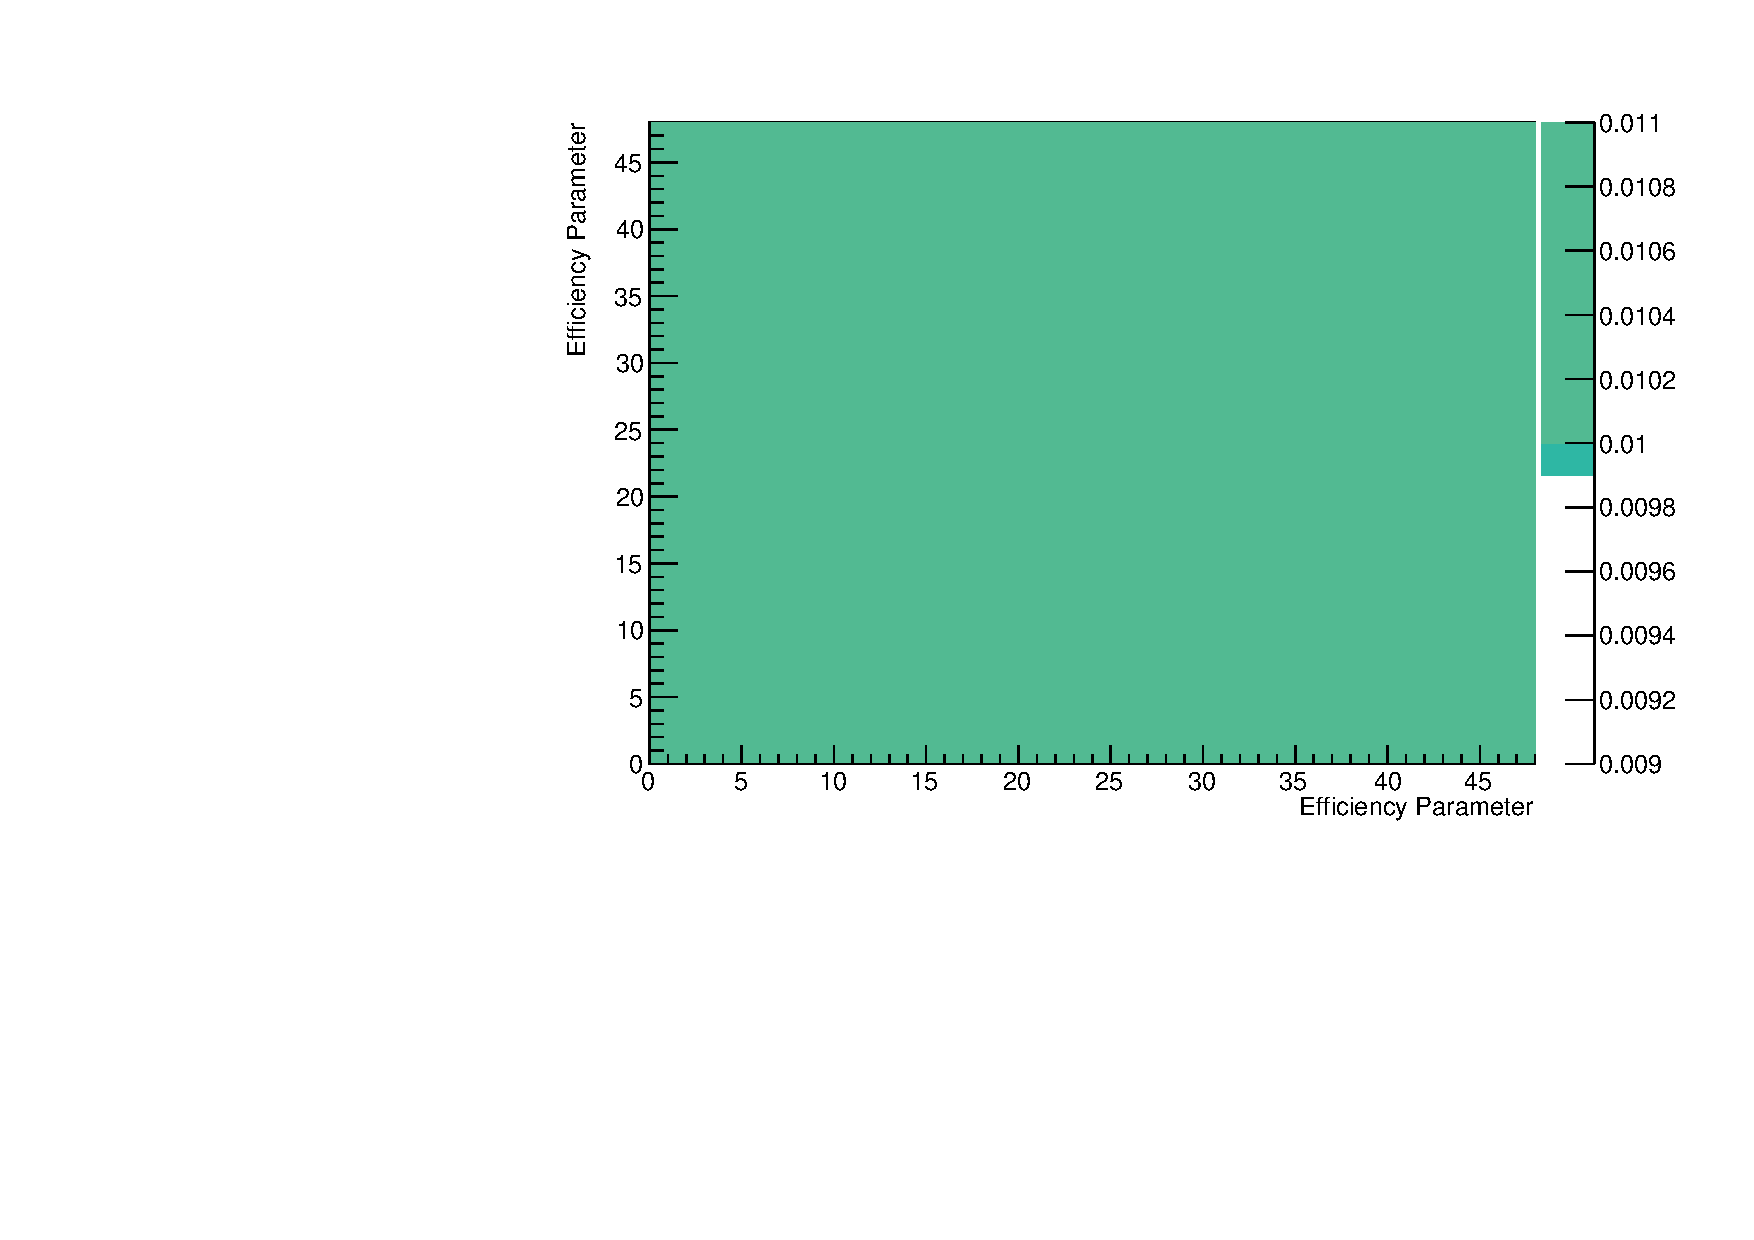
\includegraphics[width = 0.49\textwidth]{figures-chap5/efficiency_matrices/efficiency_error_matrix_48x48_type1_cor10.00pct.root.pdf}
    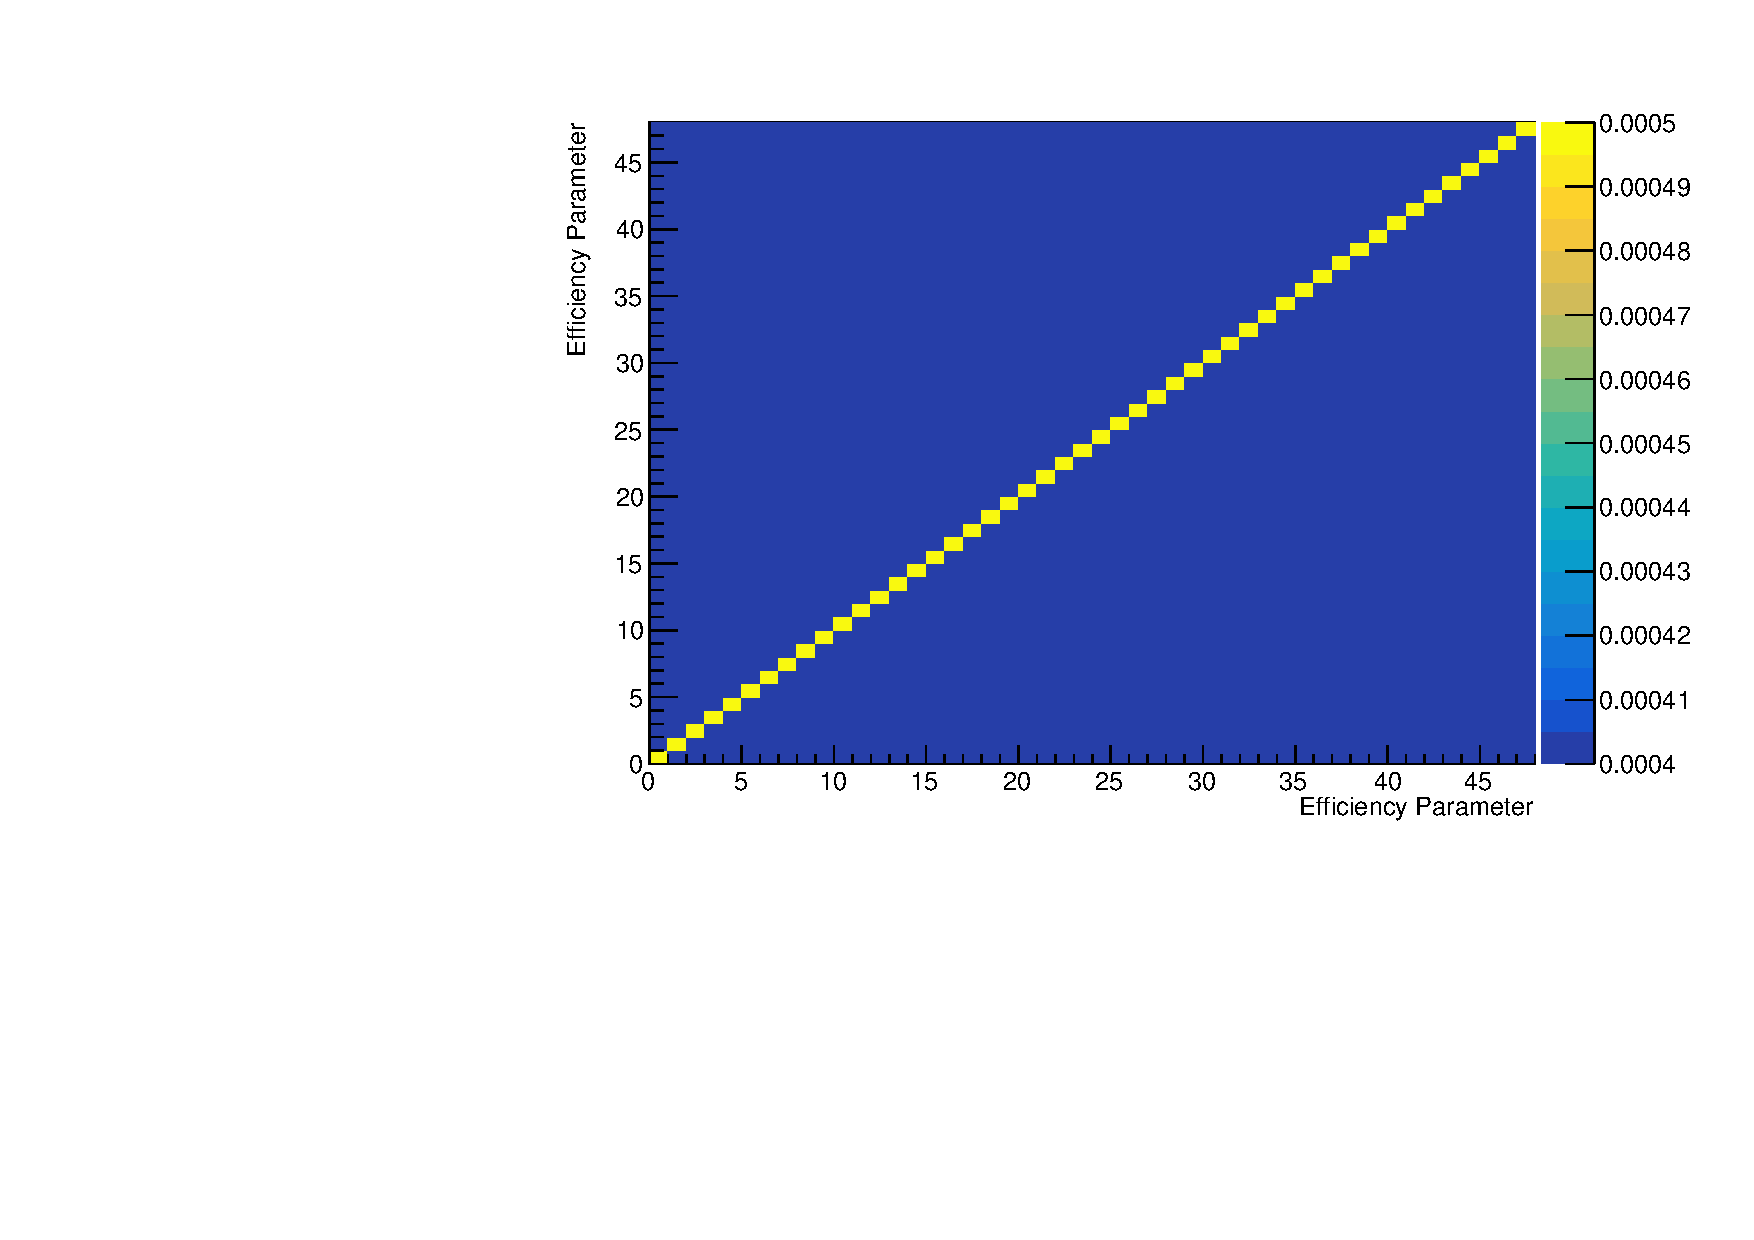
\includegraphics[width = 0.49\textwidth]{figures-chap5/efficiency_matrices/efficiency_error_matrix_48x48_type2_cor2.00pct_sbnduncor1.00pct_ubooneuncor1.00pct_icarusuncor1.00pct.root.pdf}
    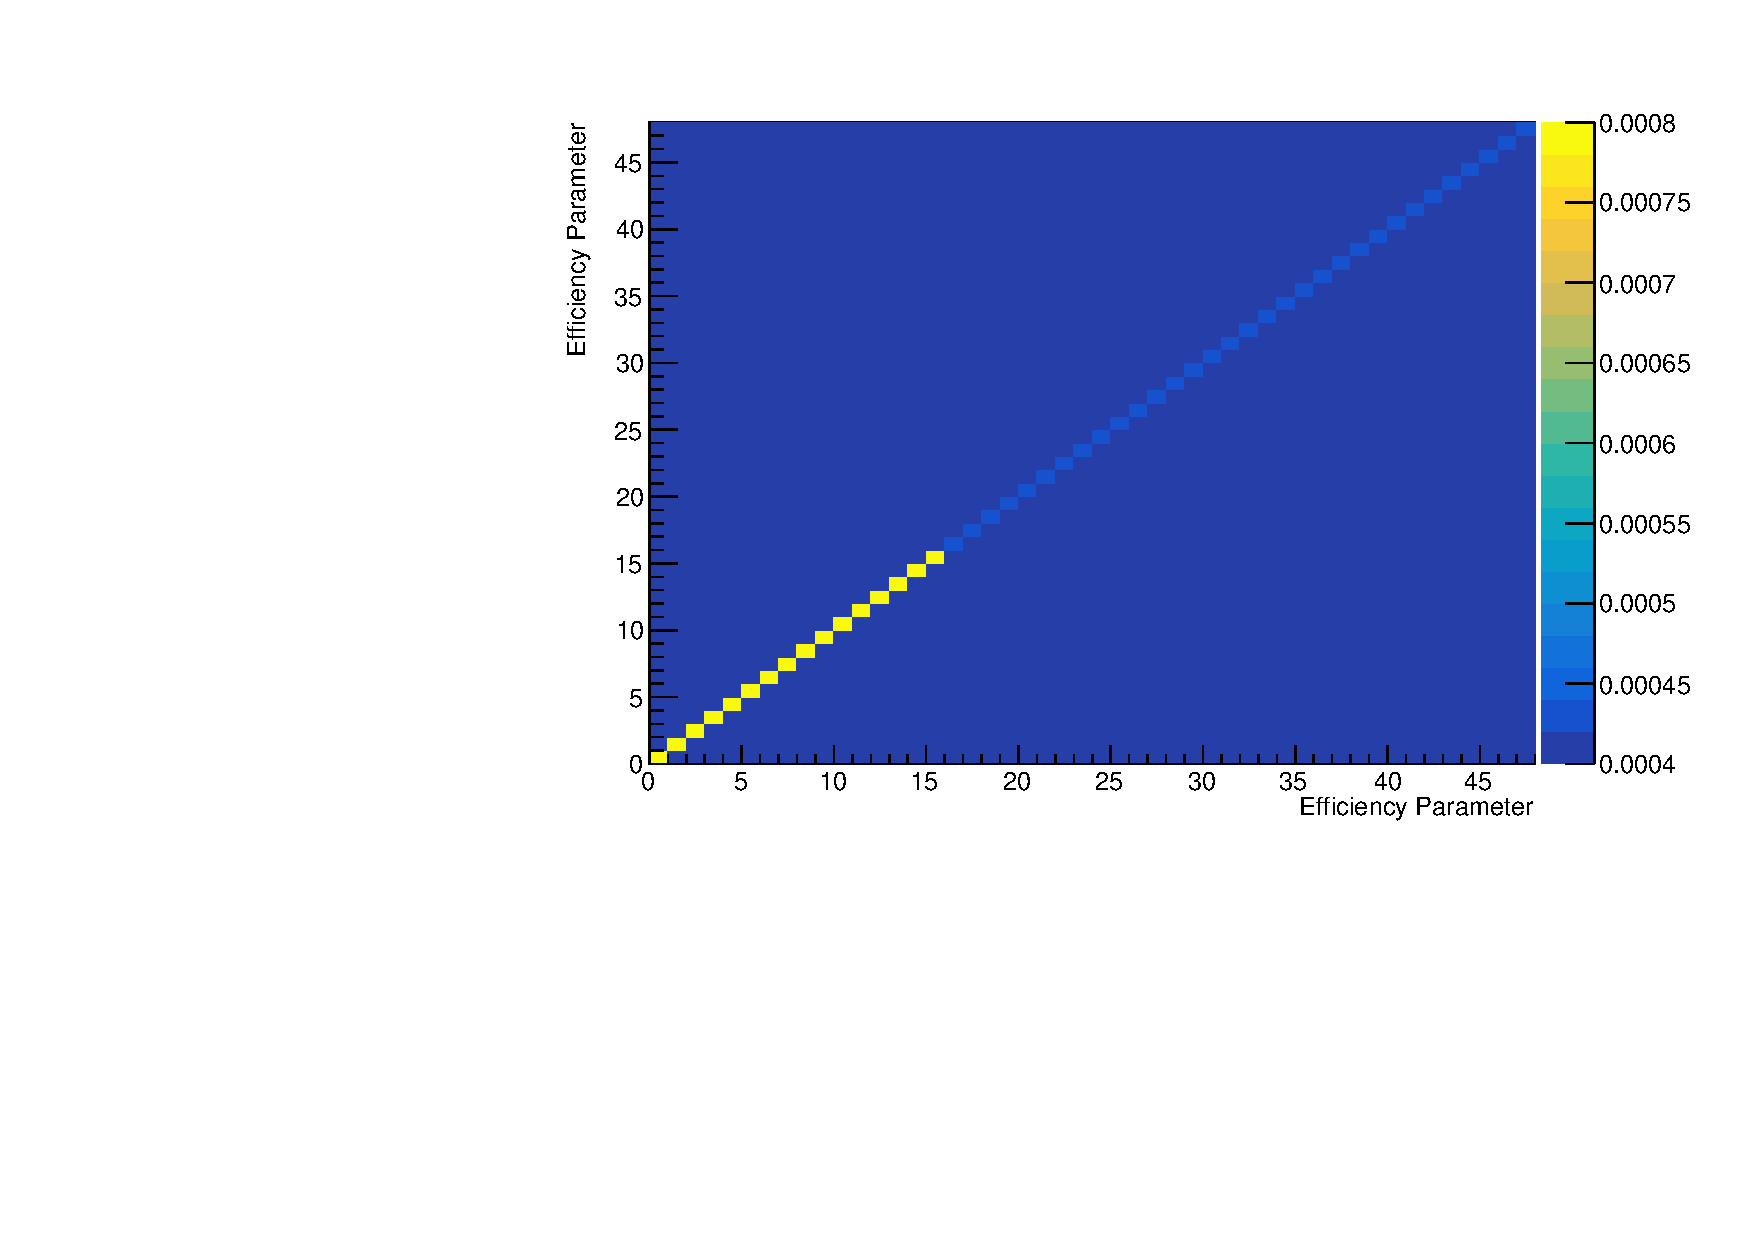
\includegraphics[width = 0.49\textwidth]{figures-chap5/efficiency_matrices/efficiency_error_matrix_48x48_type2_cor2.00pct_sbnduncor2.00pct_ubooneuncor0.50pct_icarusuncor0.50pct.root.pdf}
    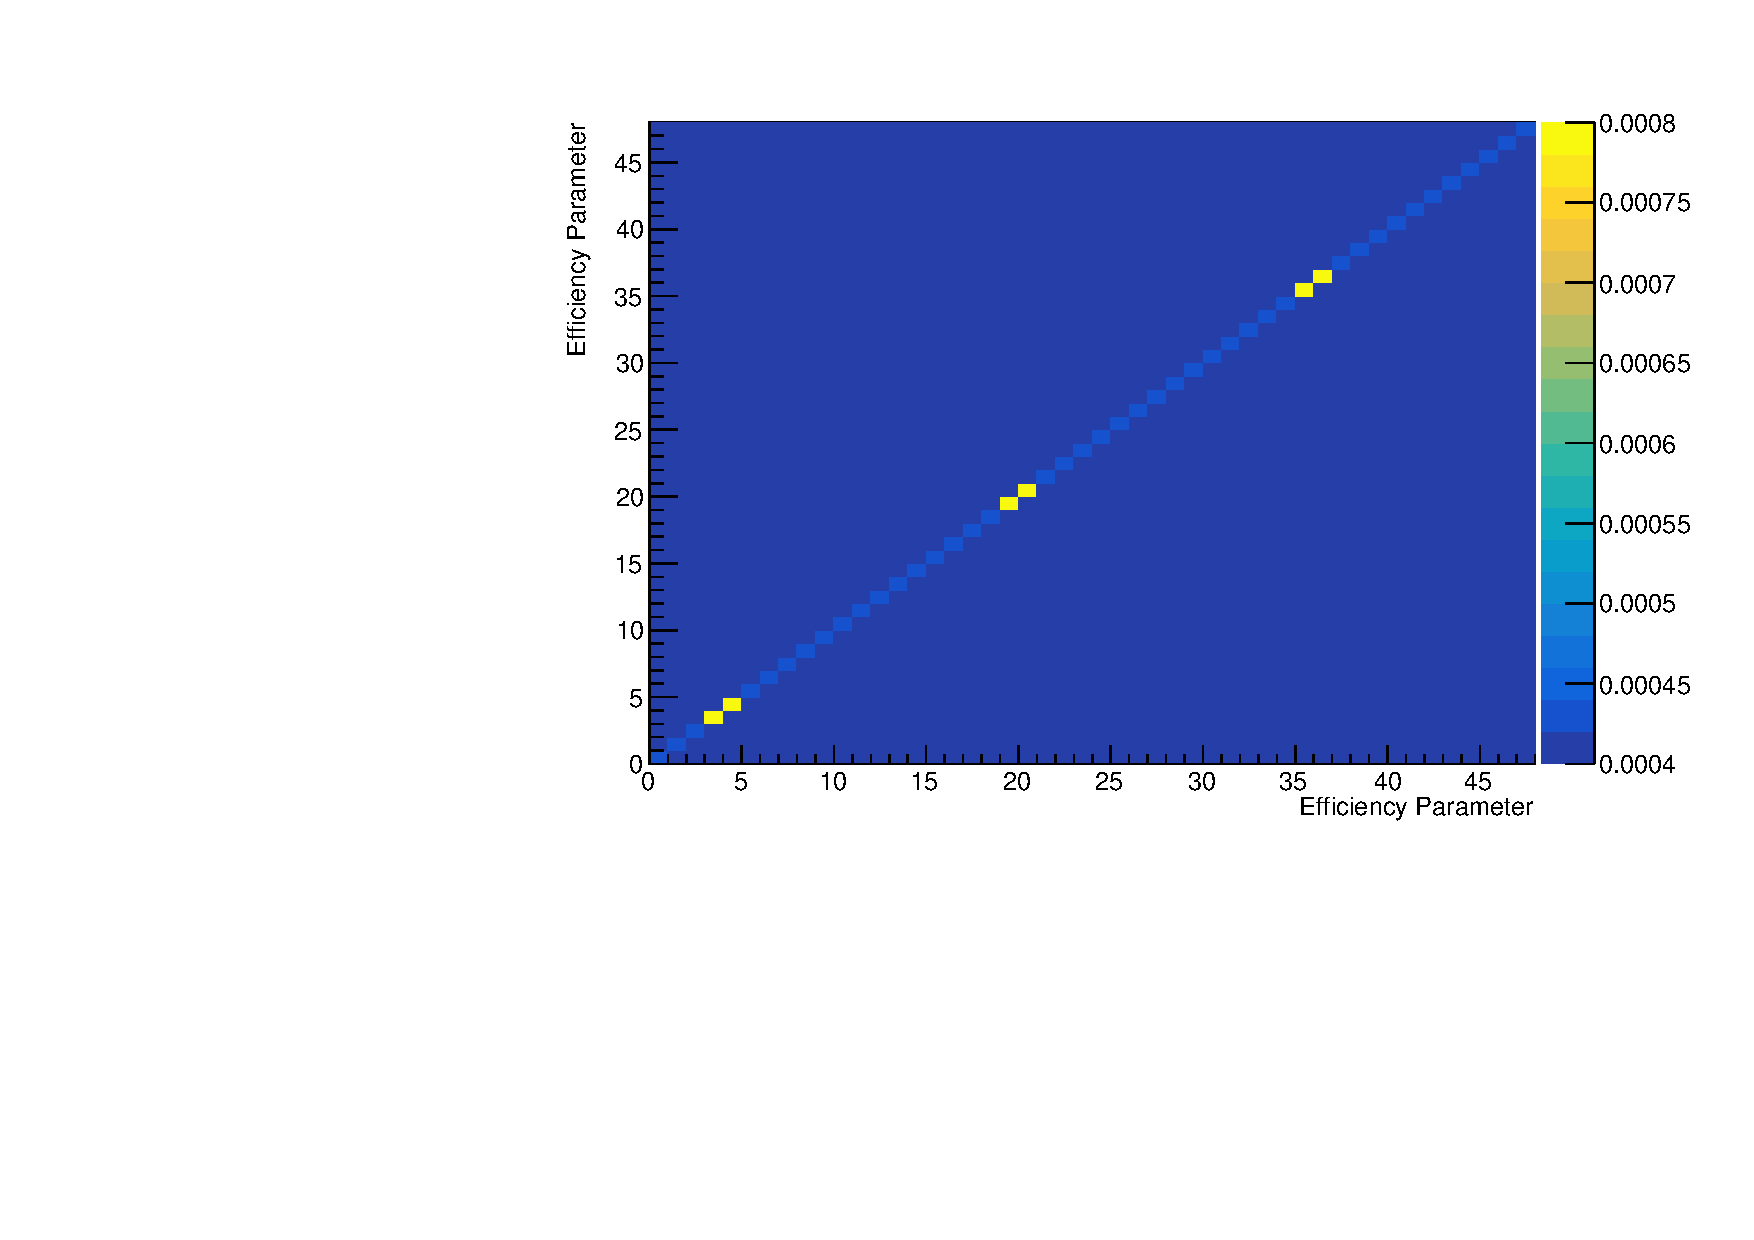
\includegraphics[width = 0.49\textwidth]{figures-chap5/efficiency_matrices/efficiency_error_matrix_48x48_type3_cor2.00pct_bulkuncor0.50pct_allpeakEnumuCCuncor2.00pct.root.pdf}
    \caption[Example efficiency uncertainty covariance matrices.]{Covariance matrices produced to investigate the effects of efficiency systematics for the \numu disappearance channel. Top left: A 10\% fully correlated error only. Top right: A 2\% fully correlated error with an additional 1\% uncorrelated error across all bins. Bottom left: A 2\% fully correlated error with an additional 2\% uncorrelated error for all \gls{sbnd} bins and a 0.5\% uncorrelated error for all \gls{microboone} and \gls{icarus} bins. Bottom right: A 2\% fully correlated error with and additional 2\% uncorrelated error for the peak energy bins (0.6 - 1.0 GeV) in each detector and a 0.5\% uncorrelated error for all other bins.}
    \label{fig:efficiency_cov_matrices}
\end{figure}




\newpage
\begin{comment}
\subsubsection*{Energy Scale Systematic}

The energy scale systematic is a global systematic to account for the fact that events are binned based on their energy. Uncertainty on the reconstructed neutrino energy means that it's possible certain events to \textit{migrate} between energy bins. Since the energy distribution of events is not flat, this migration would in general not be uniform. If the neutrino energy were to be 'dialled-up', the number of events migrating from a given bin, $b$, to the neighbouring bin, $b + 1$, would be less than the number of events migrating from bin, $b - 1$, to $b$. This effect is shown below in \FigureRef{fig:energy_scale}. 

\begin{figure}[!h]
    \centering
    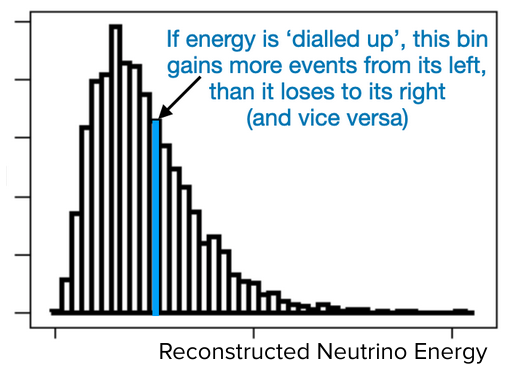
\includegraphics[width = \largefigwidth]{figures-chap5/energy_scale.png}
    \caption{Possible event migration due to uncertainty on the reconstructed neutrino energy.}
    \label{fig:energy_scale}
\end{figure}

Since the energy scale systematic is a global one, it is applied across all energy bins, for all modes, in the form a $1 \times 1$ covariance matrix.

\end{comment}

\section{Other Analysis Choices}

Two other key analysis choices are the neutrino baseline parameterisation and the binning scheme used for the kinematic variable. As is shown in \EquationRef{eqn:sterile_osc_prob}, the baseline is one of the components that drives the oscillation probability and therefore any approximations to the true baseline must be chosen such that the impact to the oscillation probability is negligible. The kinematic variable used in this analysis is the energy of the neutrino for both true and reconstructed quantities.

\subsection{Baseline}
For long baseline experiments, it's not uncommon for fitting frameworks to simply use some average value for the baseline since factors such as the interaction point in the detector or the position at which a particle decays into a neutrino would only change the average baseline for the experiment by a negligible amount. However, for short baseline experiments such as \gls{sbn}, these factors may change the baseline significantly, up to around 20\% in \gls{sbnd}. 

In an attempt to minimise computing resources, the true baseline was not initially used, but instead, several approximations to the baseline were tried. To begin with, the average baseline of each \gls{sbn} detector was used for all neutrino energies. This was calculated from the true baseline distribution of \numu events in each detector which are shown in \FigureRef{fig:numu_baseline}. Secondly, a 4-knot spline (named spline V1) for each detector was defined in order to try and better approximate the baseline. This method was improved upon by producing a spline for each of the true energy bins (named spline V2) which are defined in \SectionRef{sec:binning}. In order to establish the impact of any baseline approximations on the oscillation probability, the oscillation probability was plotted as a function of true neutrino energy with the oscillation parameters $\sin^2{2\theta_{\mu\mu}} = 0.01$ and $\Delta m^2_{41} = 50$ eV$^2$. This oscillation point was chosen to ensure that a region where rapid oscillations occur was being investigated, which would highlight the effect of any baseline choices. The oscillation probabilities as a function of energy are shown in \FigureRef{fig:baseline_osc_probability} for the four different baselines described. It was eventually decided that any approximation would be insufficient and that the true baseline should be used. 

The studies of the baseline approximations were done in the context of the \numu disappearance channel. In principle, within the \nue sample, different approximations should be applied to the different sub-samples since the baseline distribution is not the same for all the sub-samples. For example, the \numu's in the oscillated and \numu sub-samples will both mainly be the result of pion decays whereas the \nue's in the intrinsic sub-sample will have a larger contribution from kaon and secondary muon decays. Pions and kaons have different lifetimes which coupled with the contribution from the decay of secondary particles means that the baseline distribution of the oscillated and \numu sub-sample will be different to that of the intrinsic \nue sub-sample. This was never done since it was decided that the true baseline should be used. The baseline distributions for the intrinsic \nue, oscillated $\nu$ and the overall \nue sample from combining all the sub-samples together are shown in \FigureRef{fig:nue_intrinsic_baseline}, \FigureRef{fig:nue_osc_baseline} and \FigureRef{fig:nue_baseline} respectively for each of the \gls{sbn} detectors. It should be noted that the baseline distributions for oscillated \nue sample from \FigureRef{fig:nue_osc_baseline} and the \numu sample from \FigureRef{fig:numu_baseline} are comparable. This is due to the initial parameters describing the oscillated sample being the same as for the \numu sample. The only difference being the neutrino oscillations from \numu to \nue which is not something that affects the baseline.

\begin{comment}
\begin{figure}[!h]
    \centering
    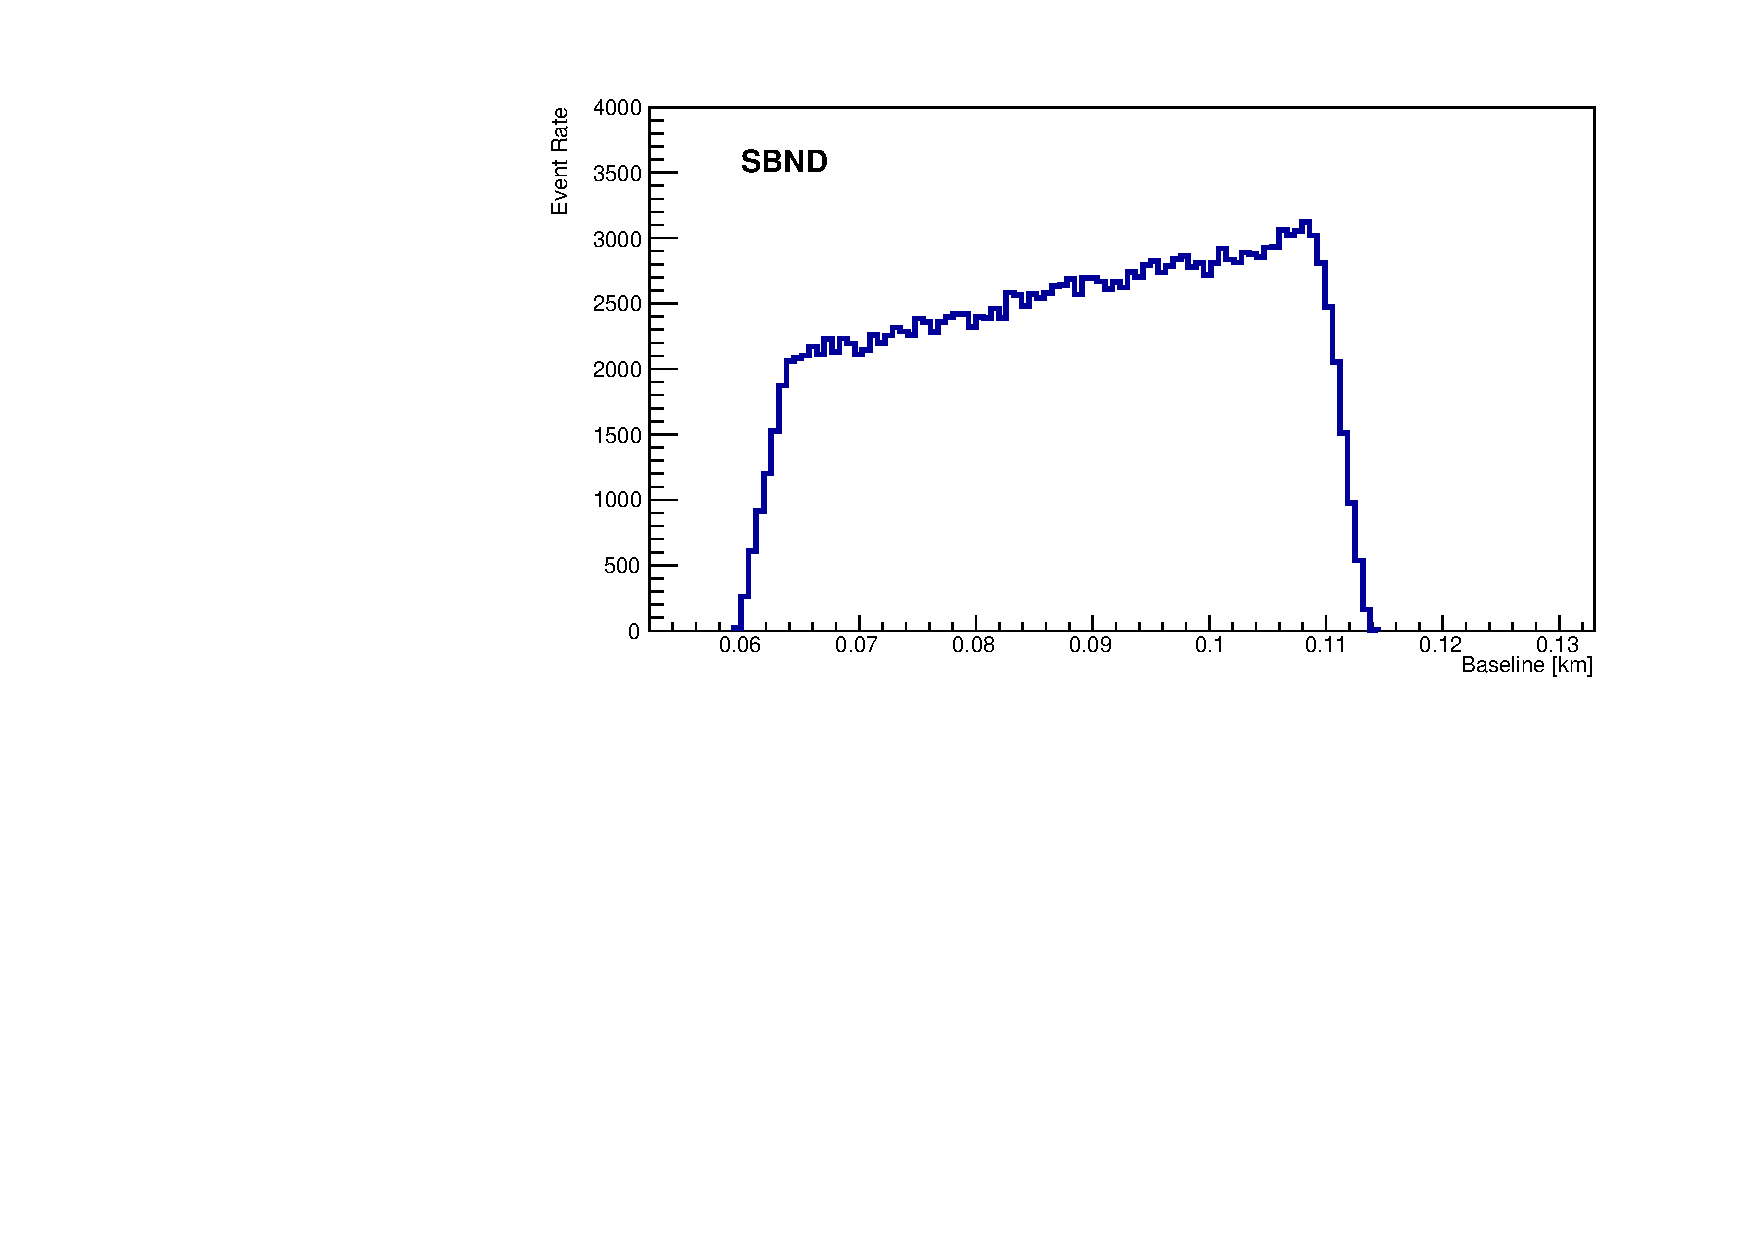
\includegraphics[width = 0.32\textwidth]{figures-chap5/SBND_numu.pdf}
    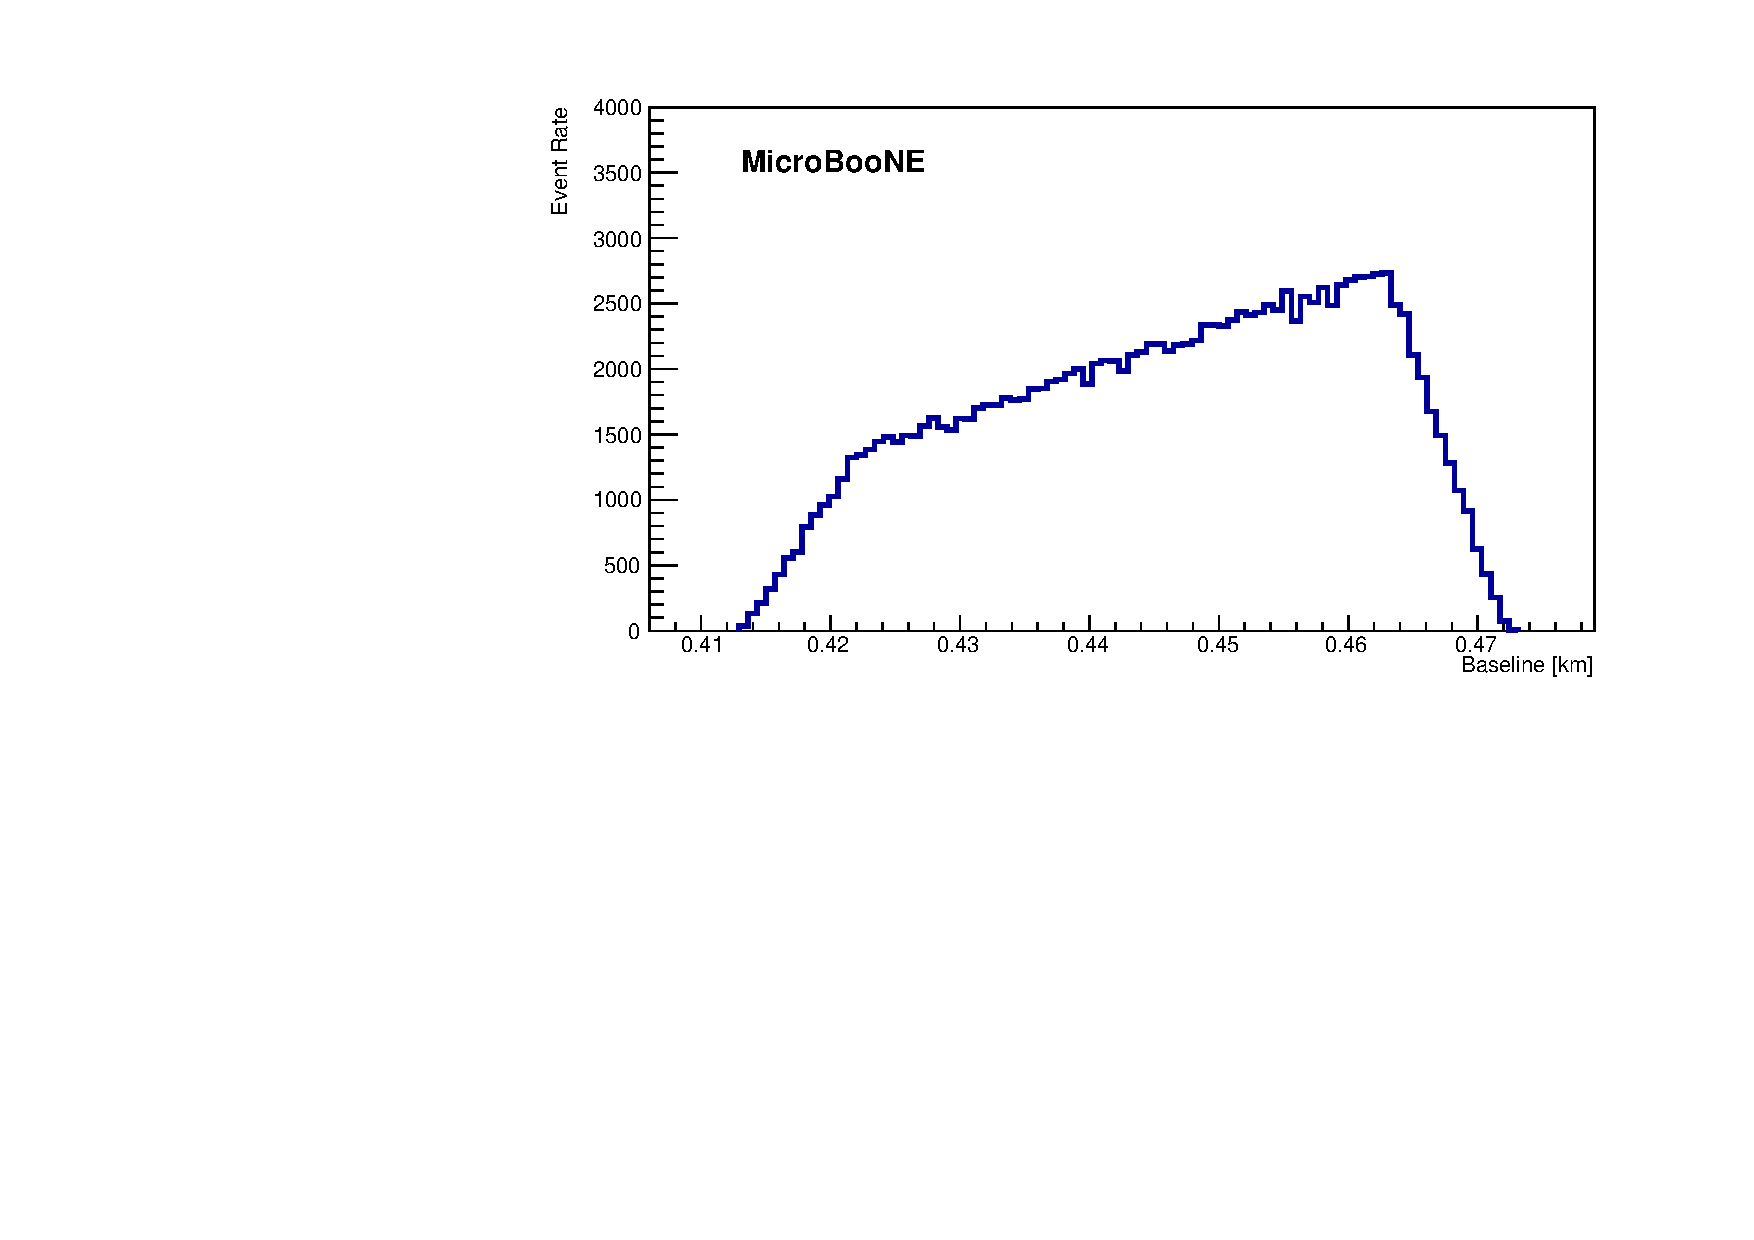
\includegraphics[width = 0.32\textwidth]{figures-chap5/MicroBooNE_numu.pdf}
    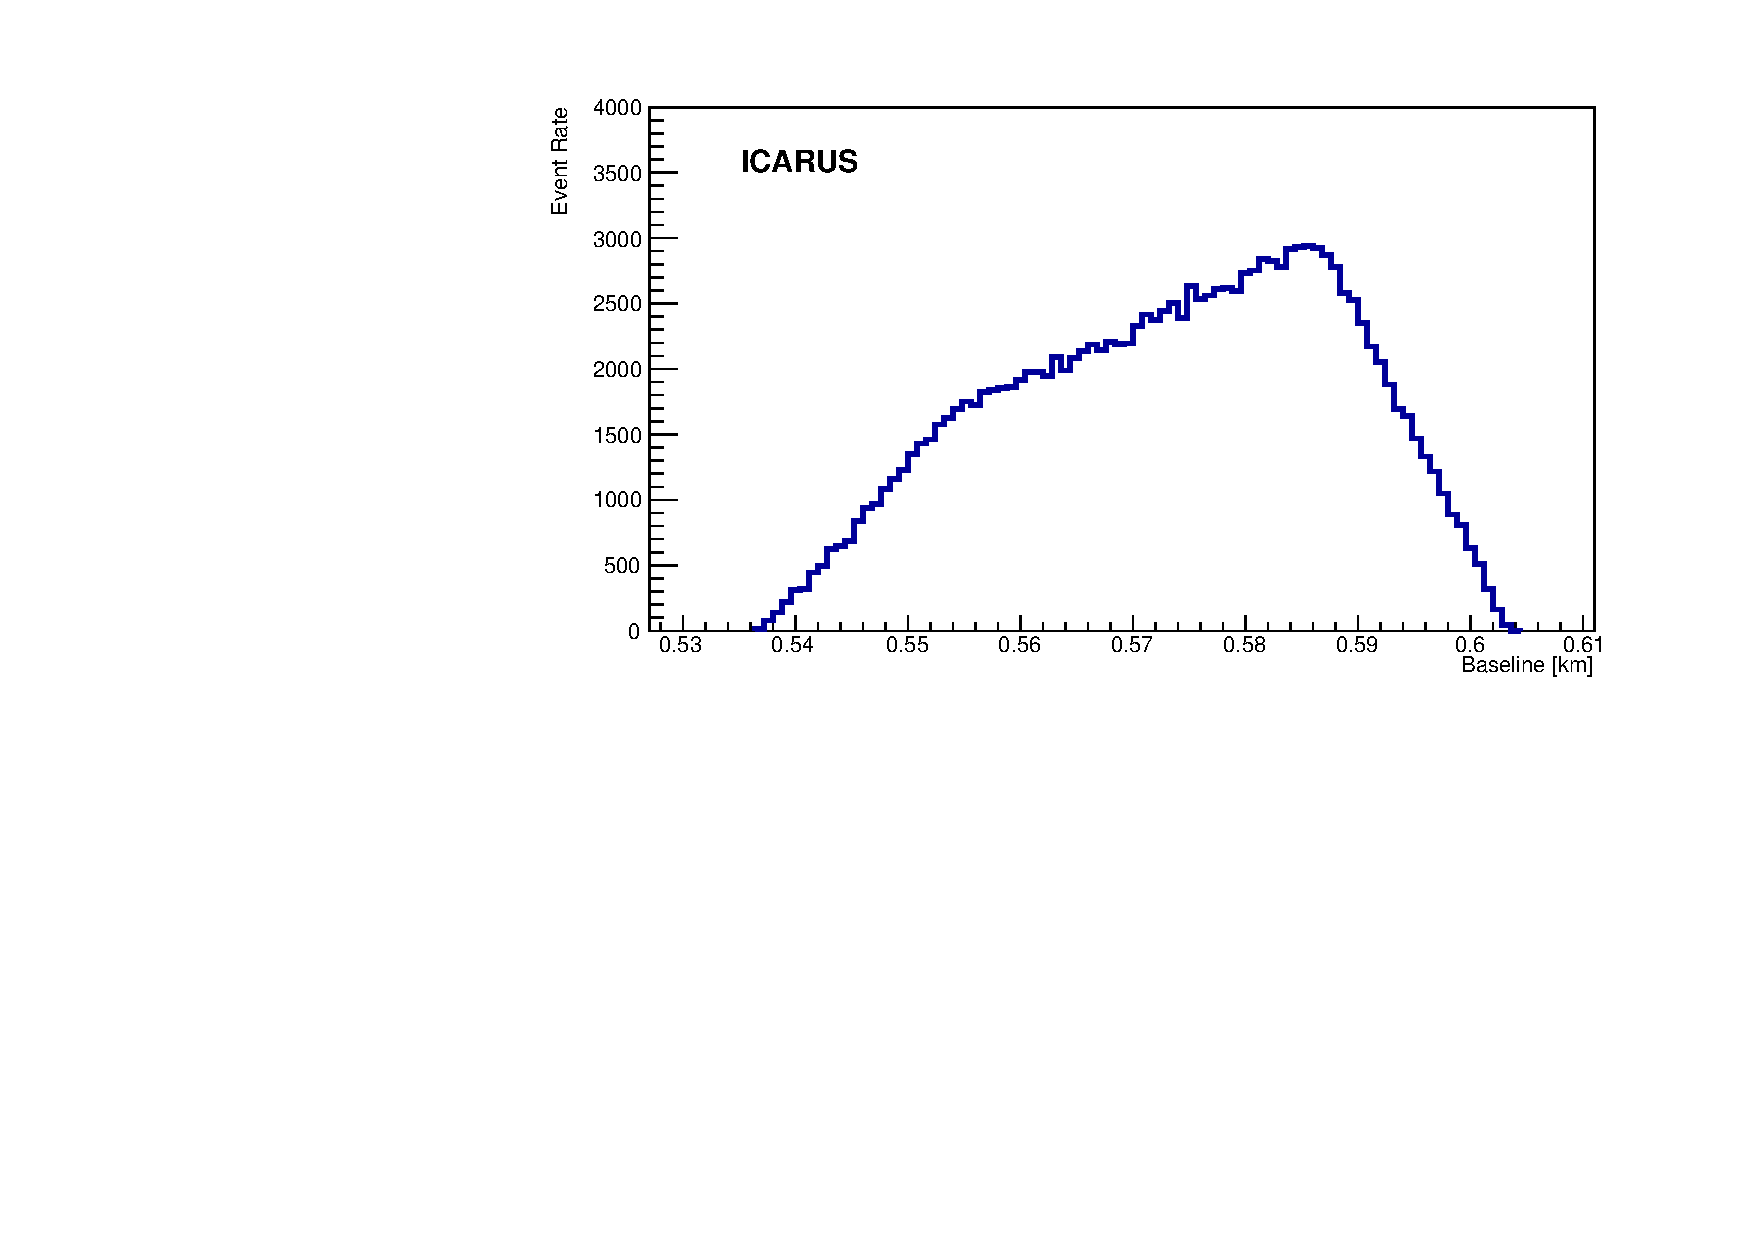
\includegraphics[width = 0.32\textwidth]{figures-chap5/ICARUS_numu.pdf}
    \caption{The baseline distribution of events in the \numu sample for each of the \gls{sbn} detectors.}
    \label{fig:numu_baseline}
\end{figure}
\end{comment}

\begin{figure}[h!]
    \centering
    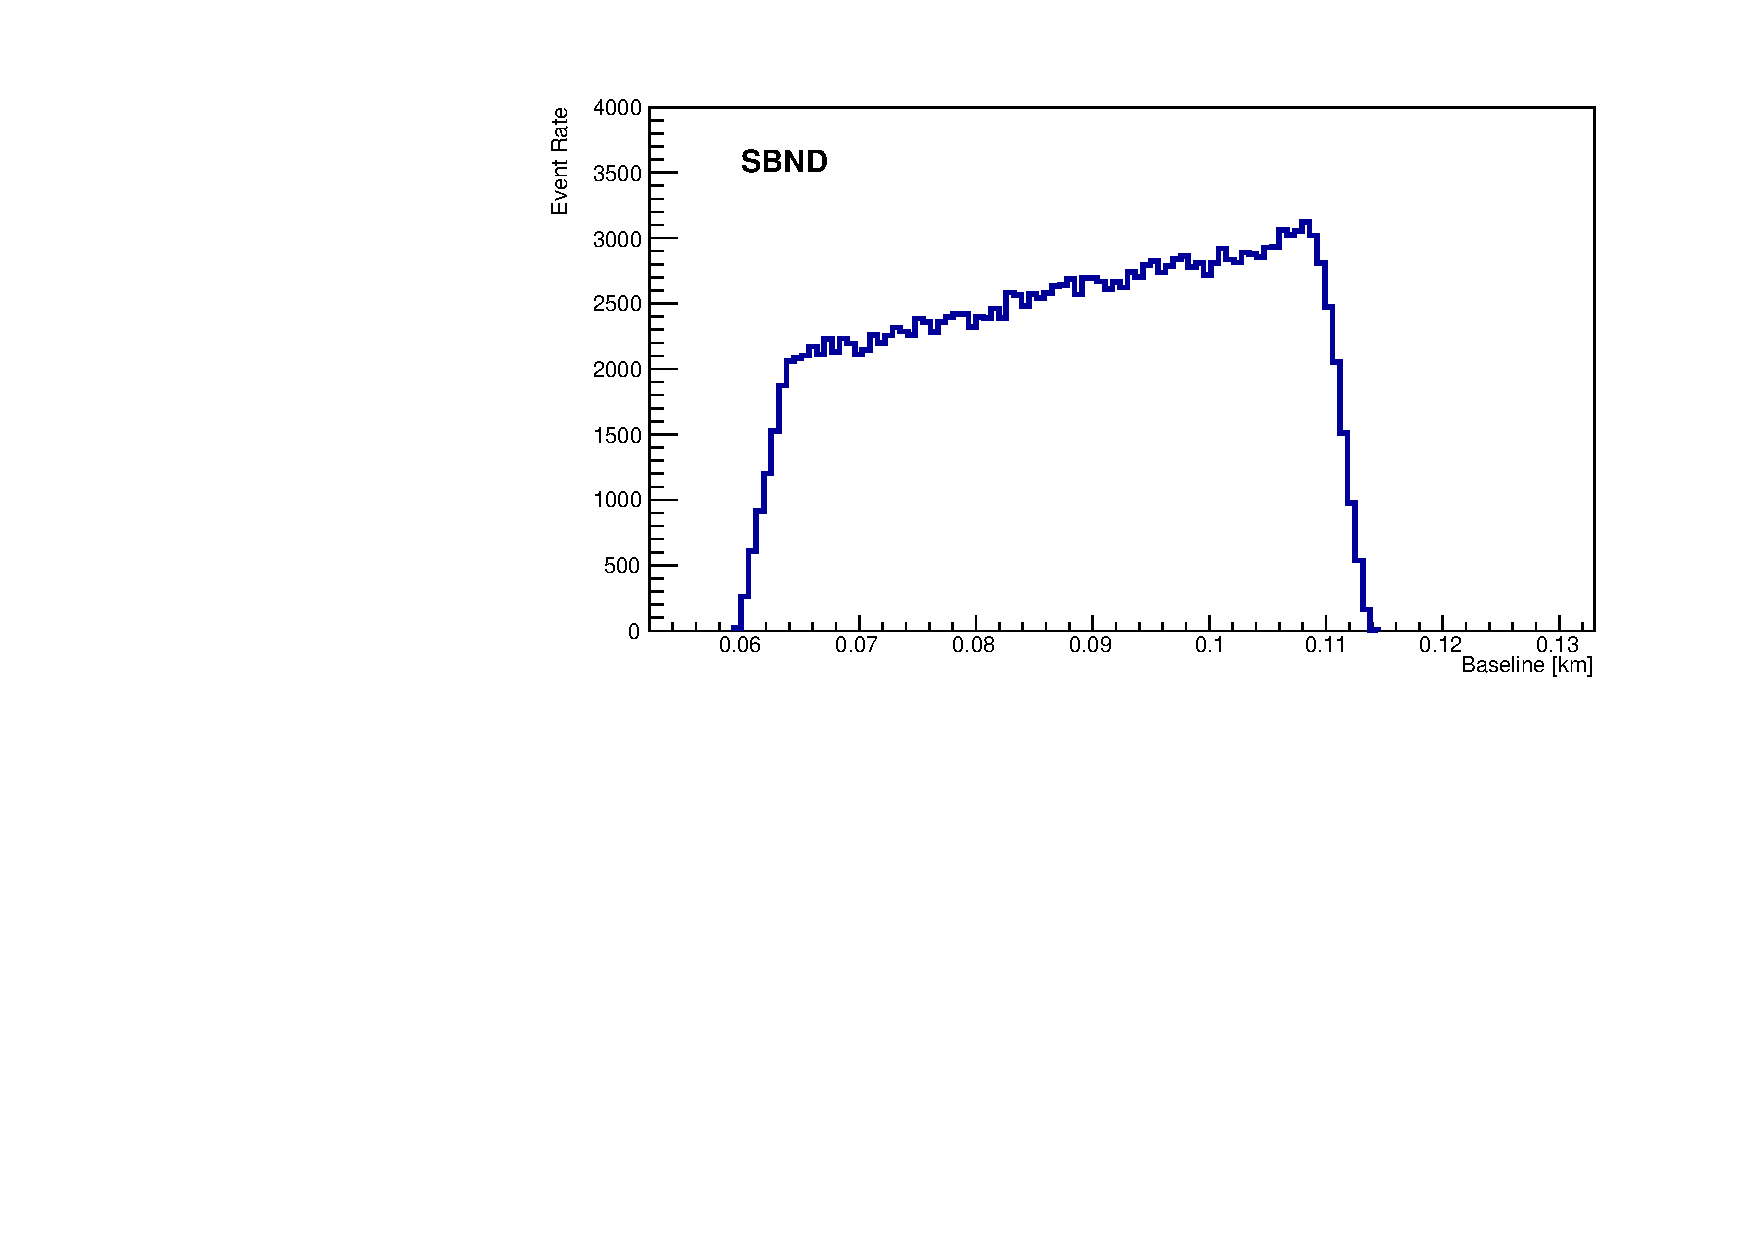
\includegraphics[width = 0.49\textwidth]{figures-chap5/SBND_numu.pdf}
    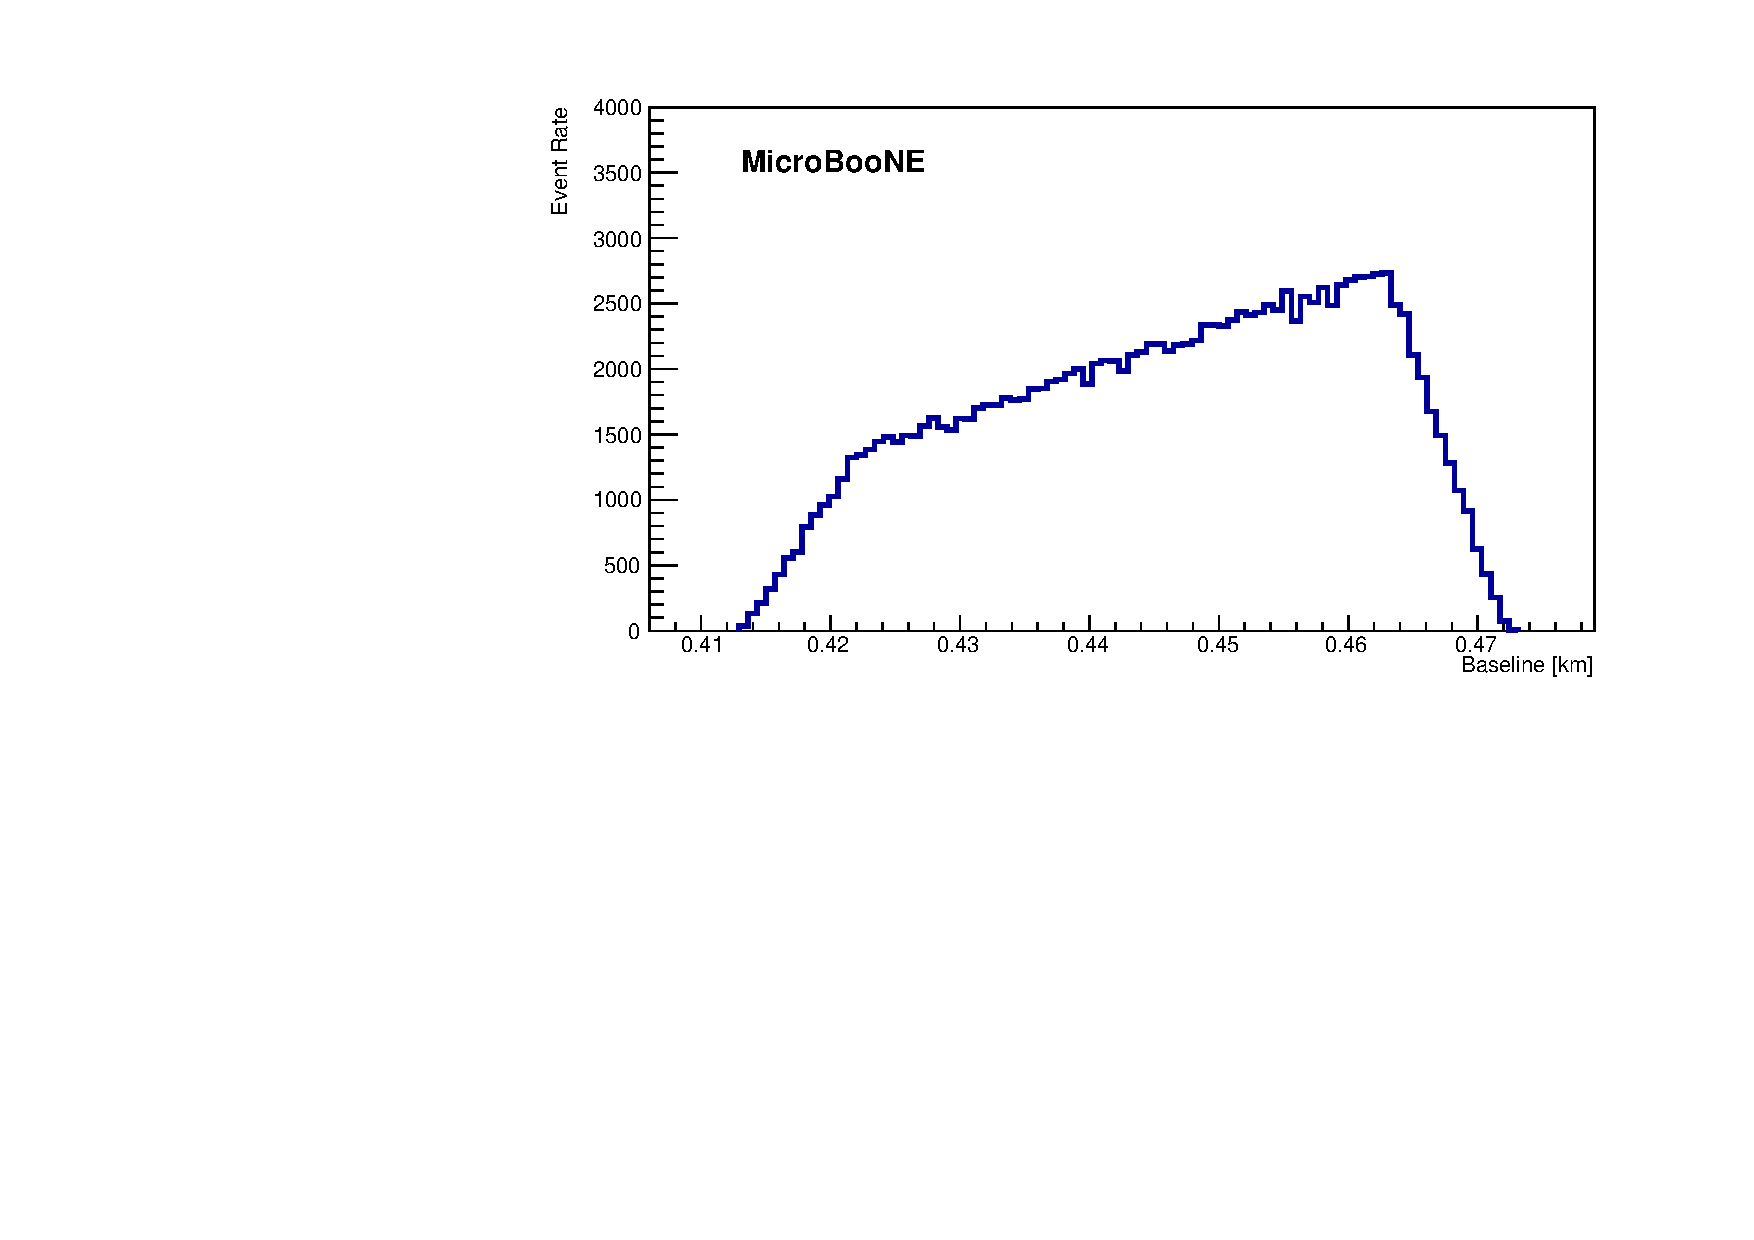
\includegraphics[width = 0.49\textwidth]{figures-chap5/MicroBooNE_numu.pdf}
    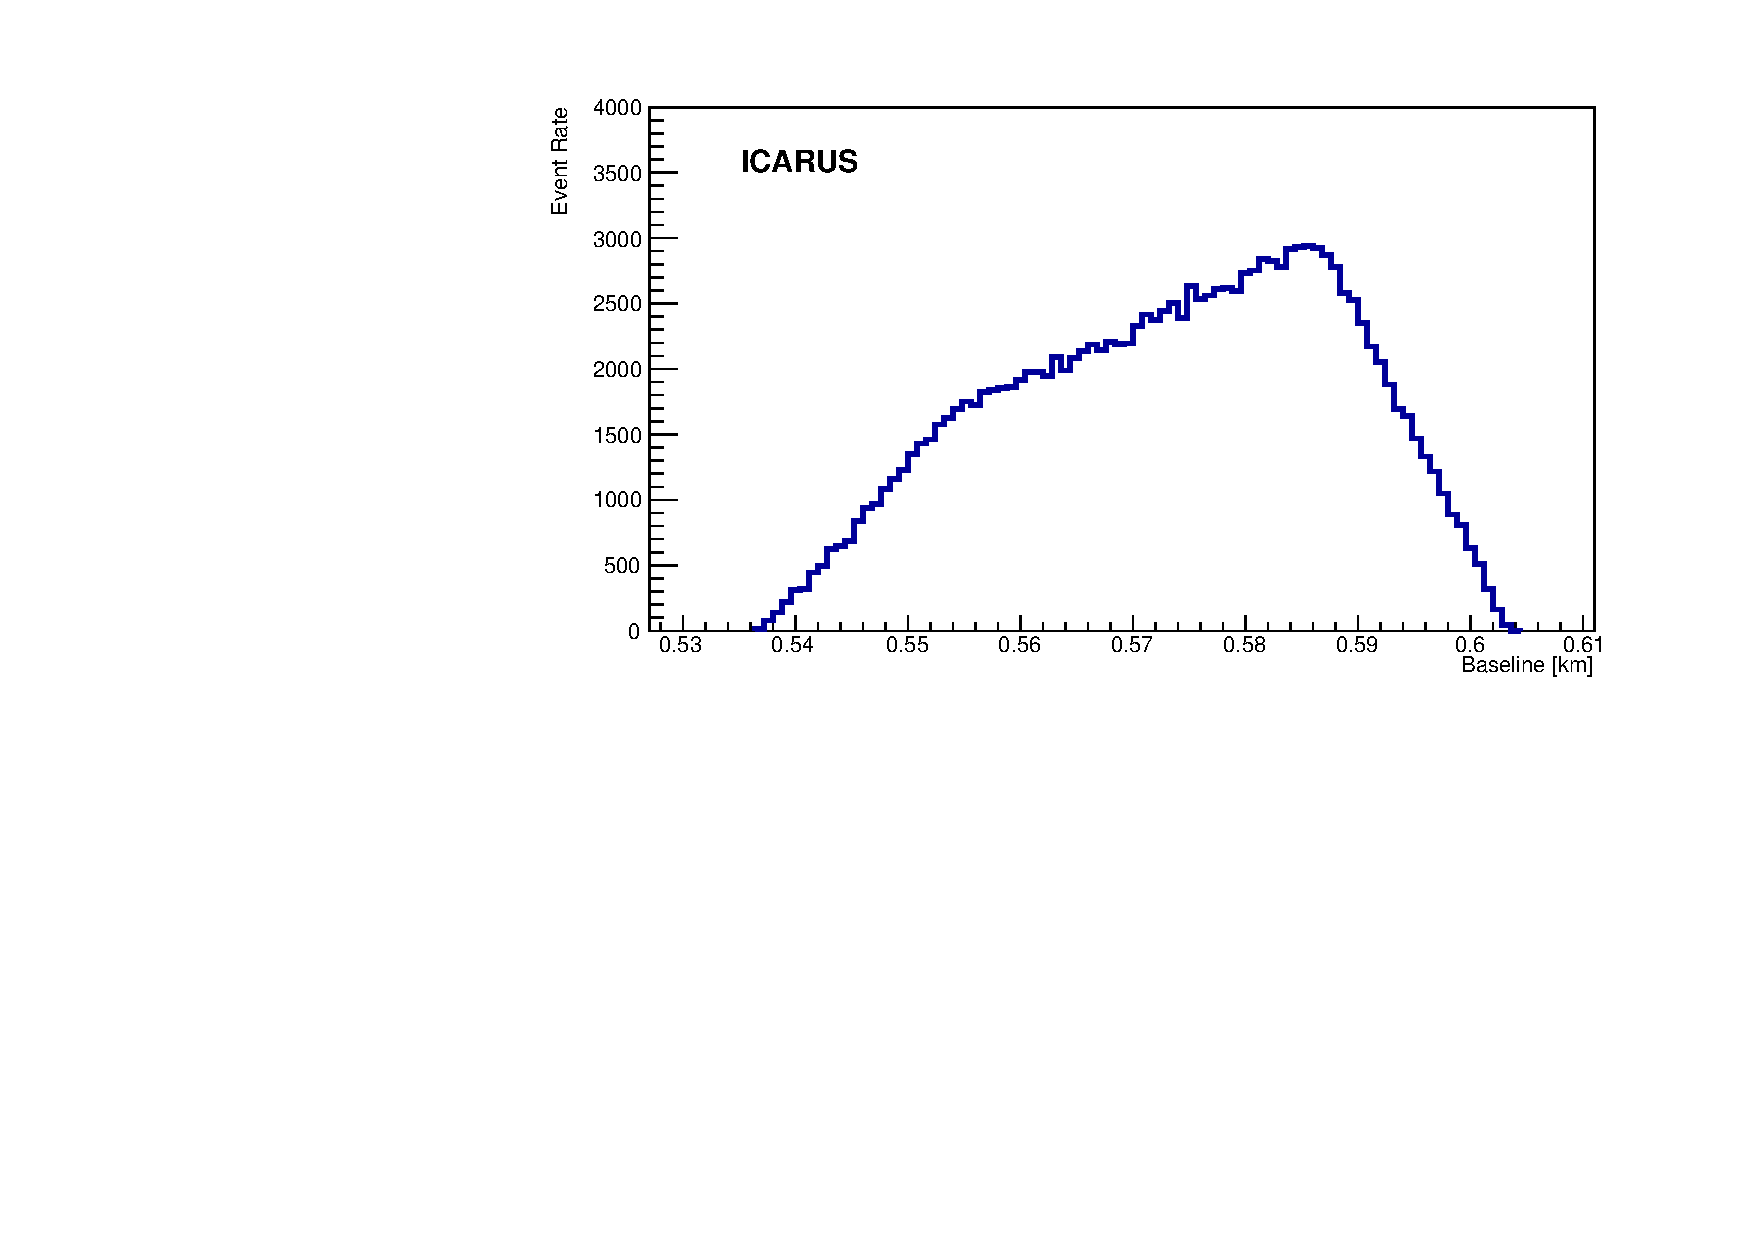
\includegraphics[width = 0.49\textwidth]{figures-chap5/ICARUS_numu.pdf}
    \captionsetup{width=0.45\textwidth}
    \parbox[b]{0.49\textwidth}%
  {
    \caption{The baseline distribution of events in the \numu sample for each of the \gls{sbn} detectors. \\\phantom{.}\\}
    \label{fig:numu_baseline}}
\end{figure}



\begin{figure}[!h]
    \centering
    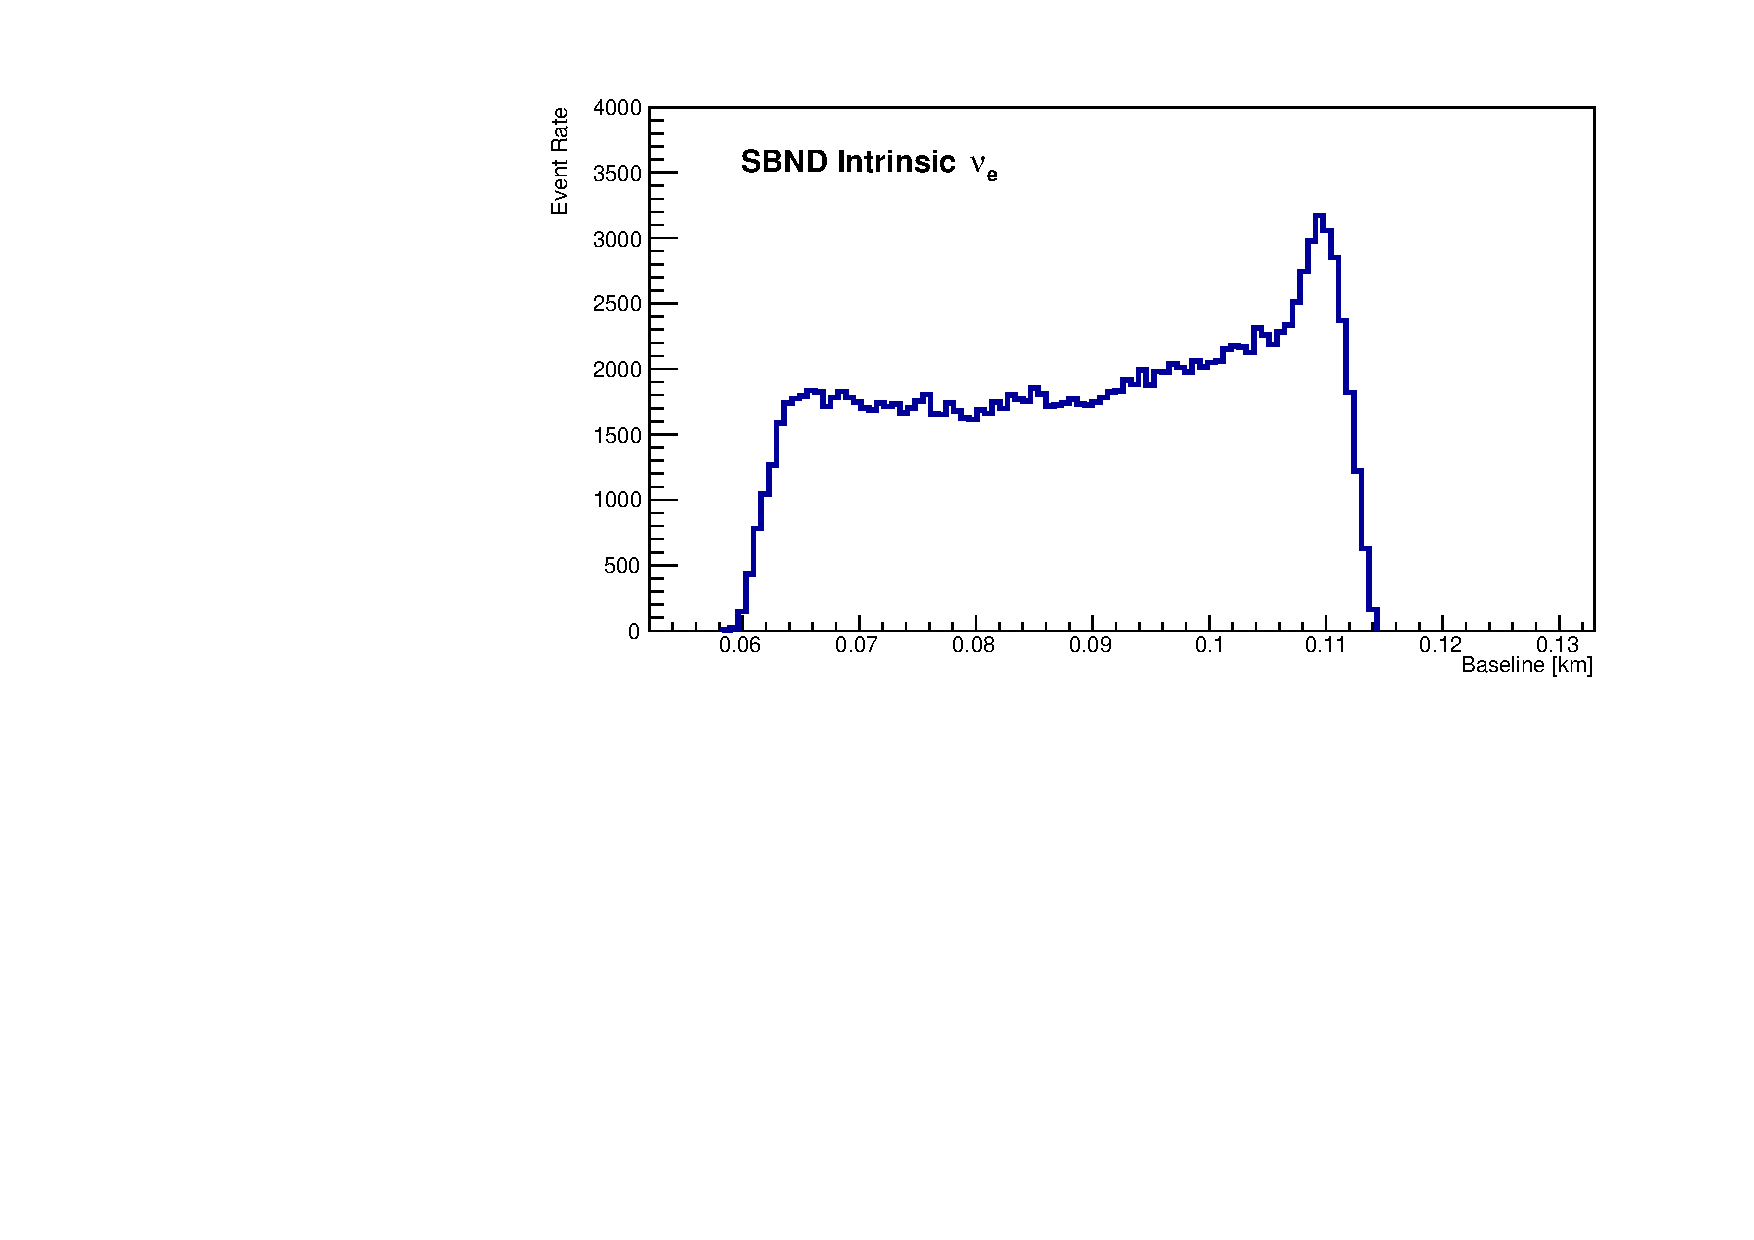
\includegraphics[width = 0.49\textwidth]{figures-chap5/SBND_intrinsic_nue.pdf}
    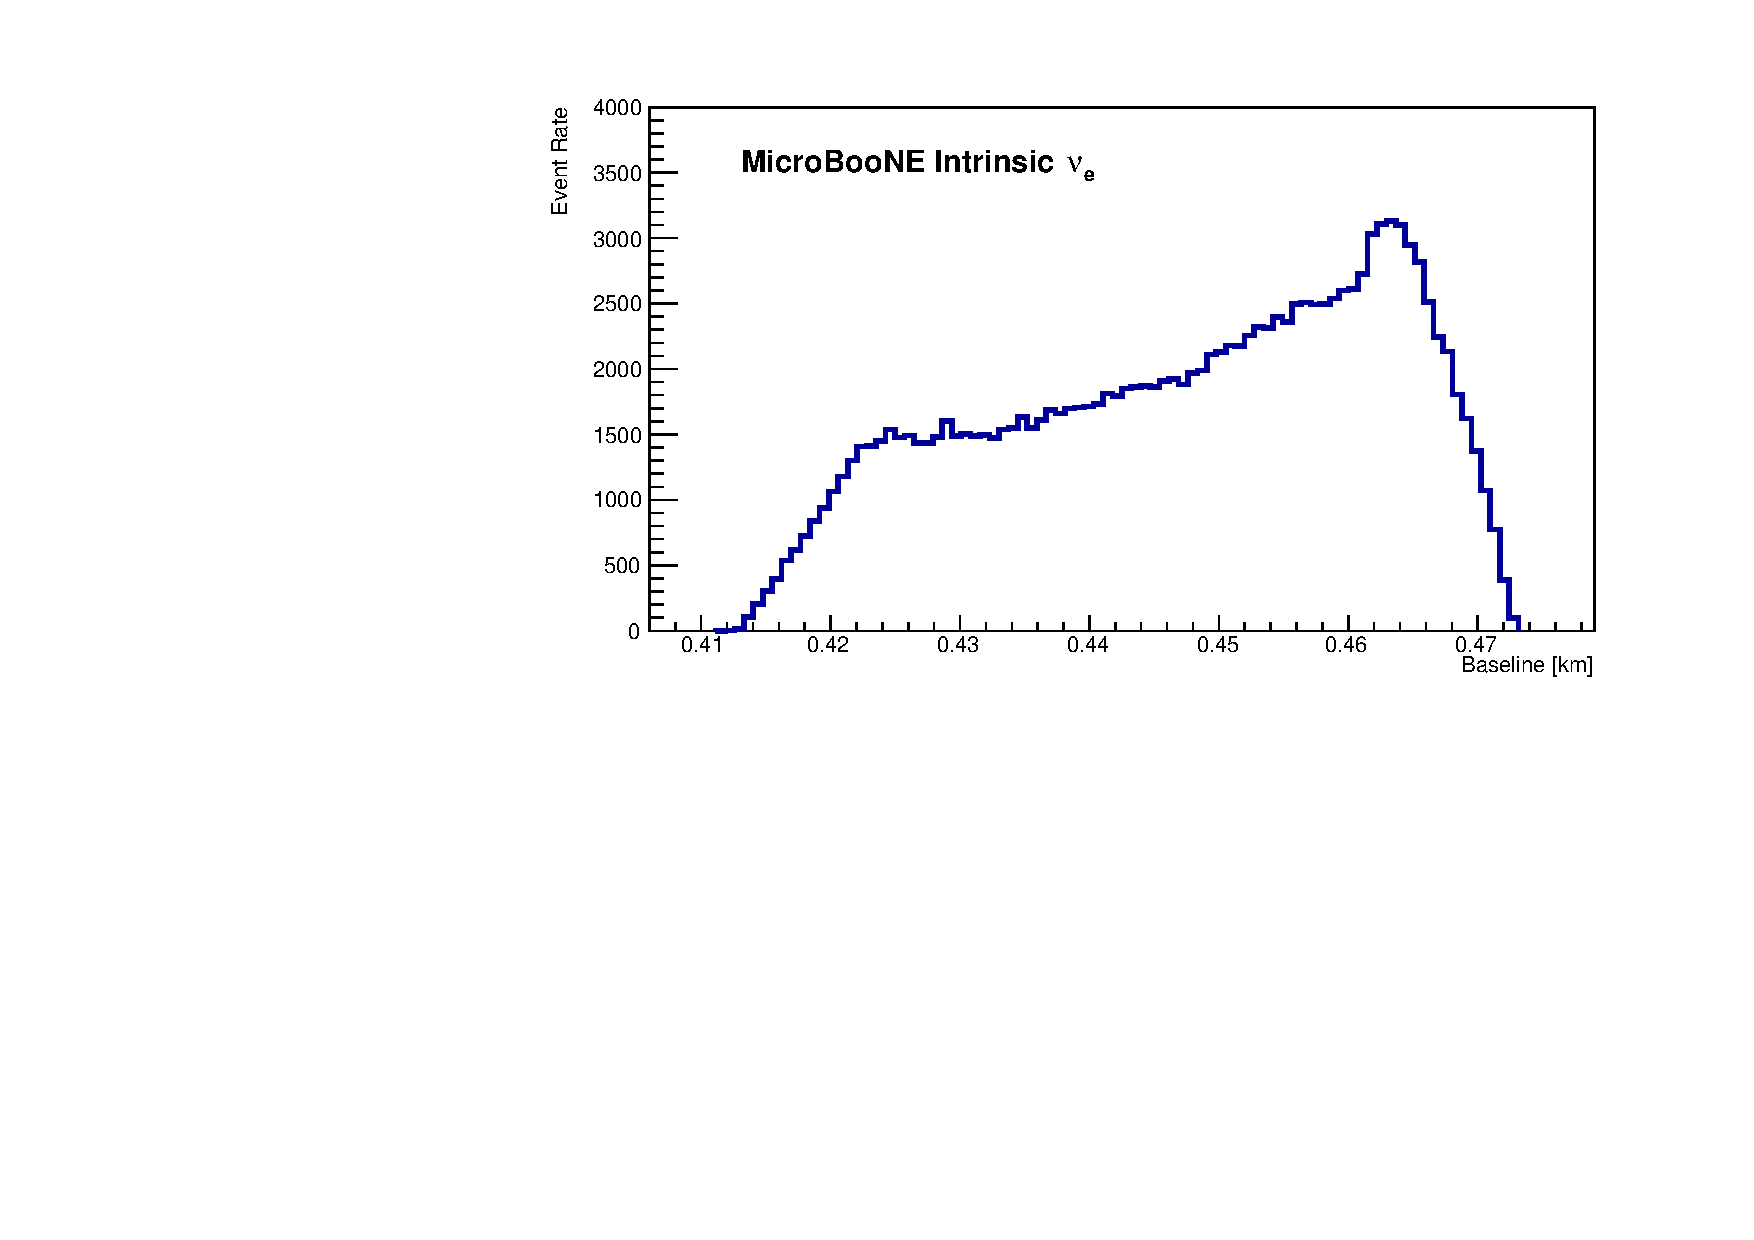
\includegraphics[width = 0.49\textwidth]{figures-chap5/MicroBooNE_intrinsic_nue.pdf}
    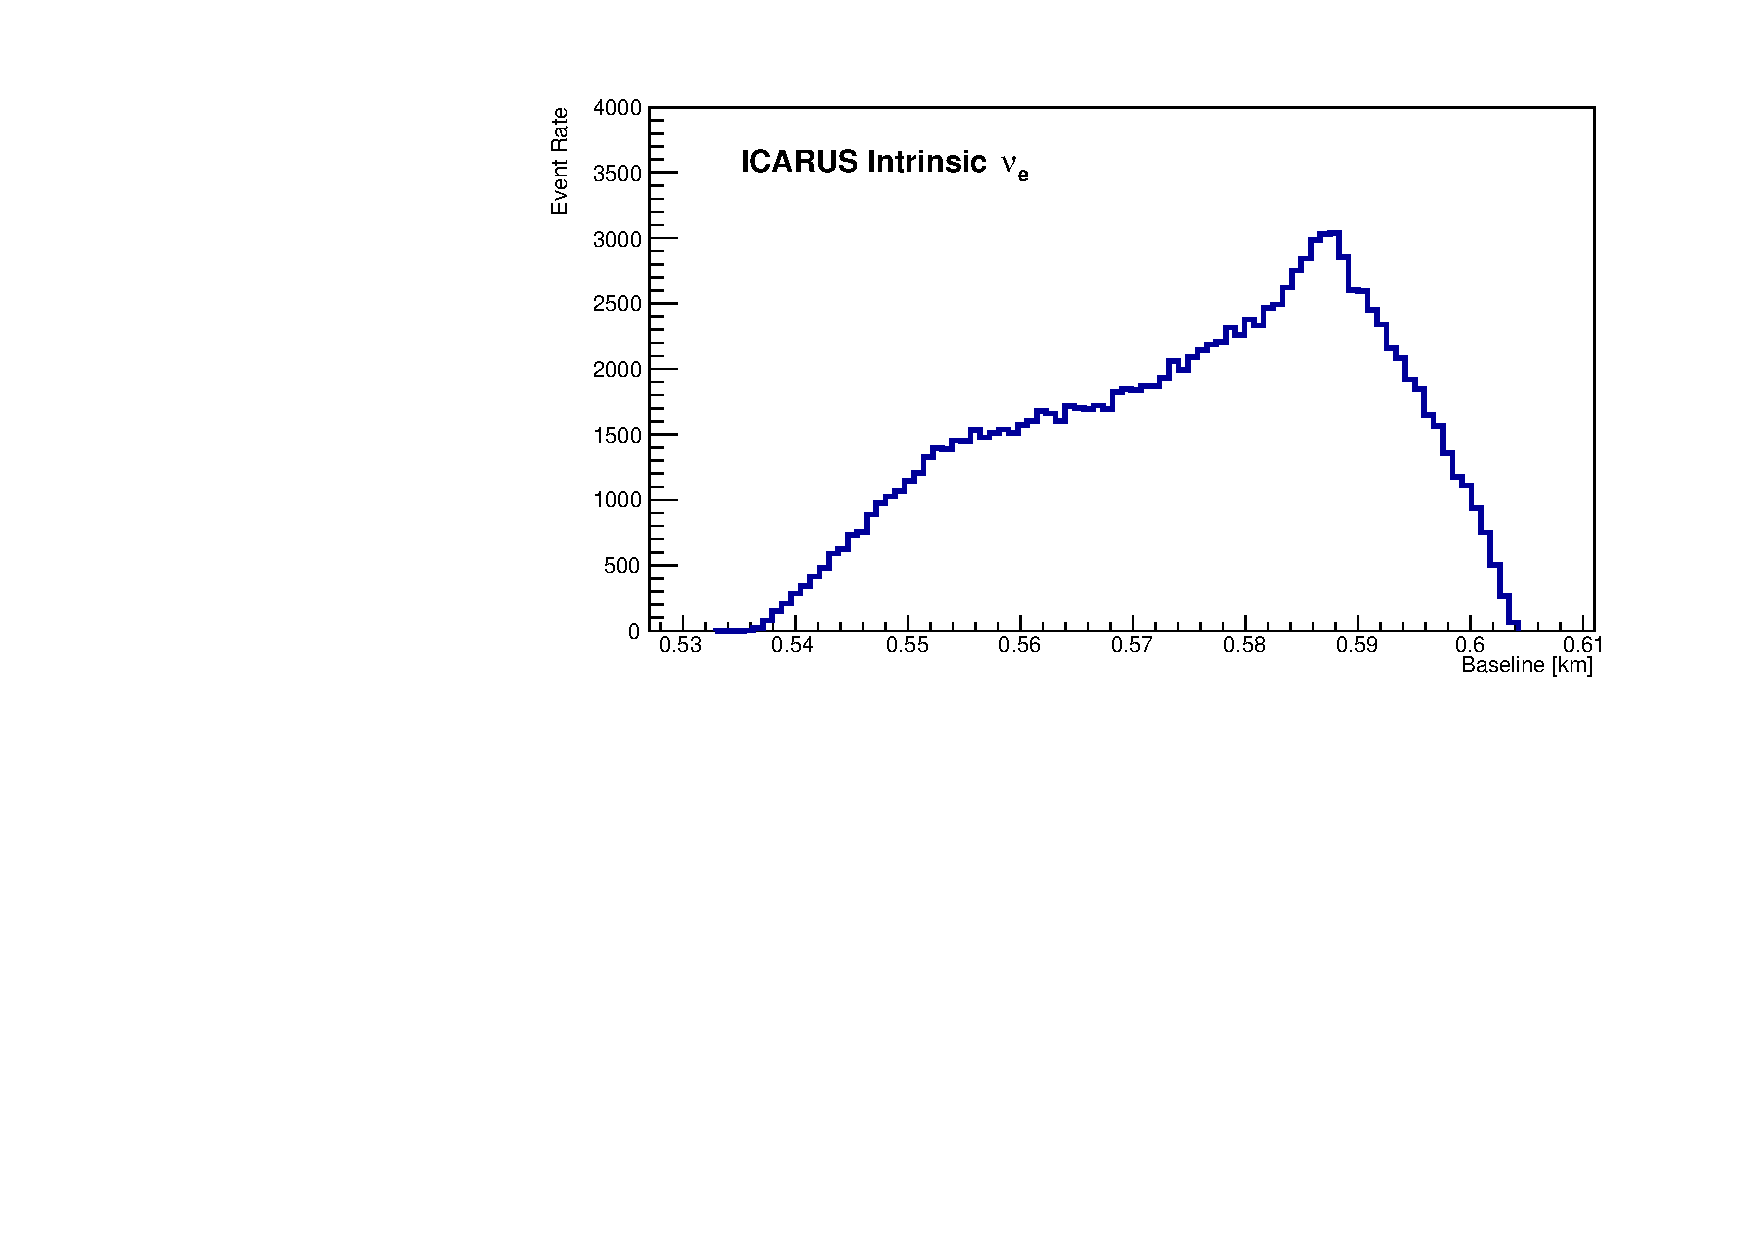
\includegraphics[width = 0.49\textwidth]{figures-chap5/ICARUS_intrinsic_nue.pdf} 
    \captionsetup{width=0.45\textwidth}
    \parbox[b]{0.49\textwidth}%
    {
    \caption{The baseline distribution of events in the intrinsic \nue sample for each of the \gls{sbn} detectors. \\\phantom{.}\\}
    \label{fig:nue_intrinsic_baseline}
    }
  \end{figure}
  
  \begin{figure}
    \centering
    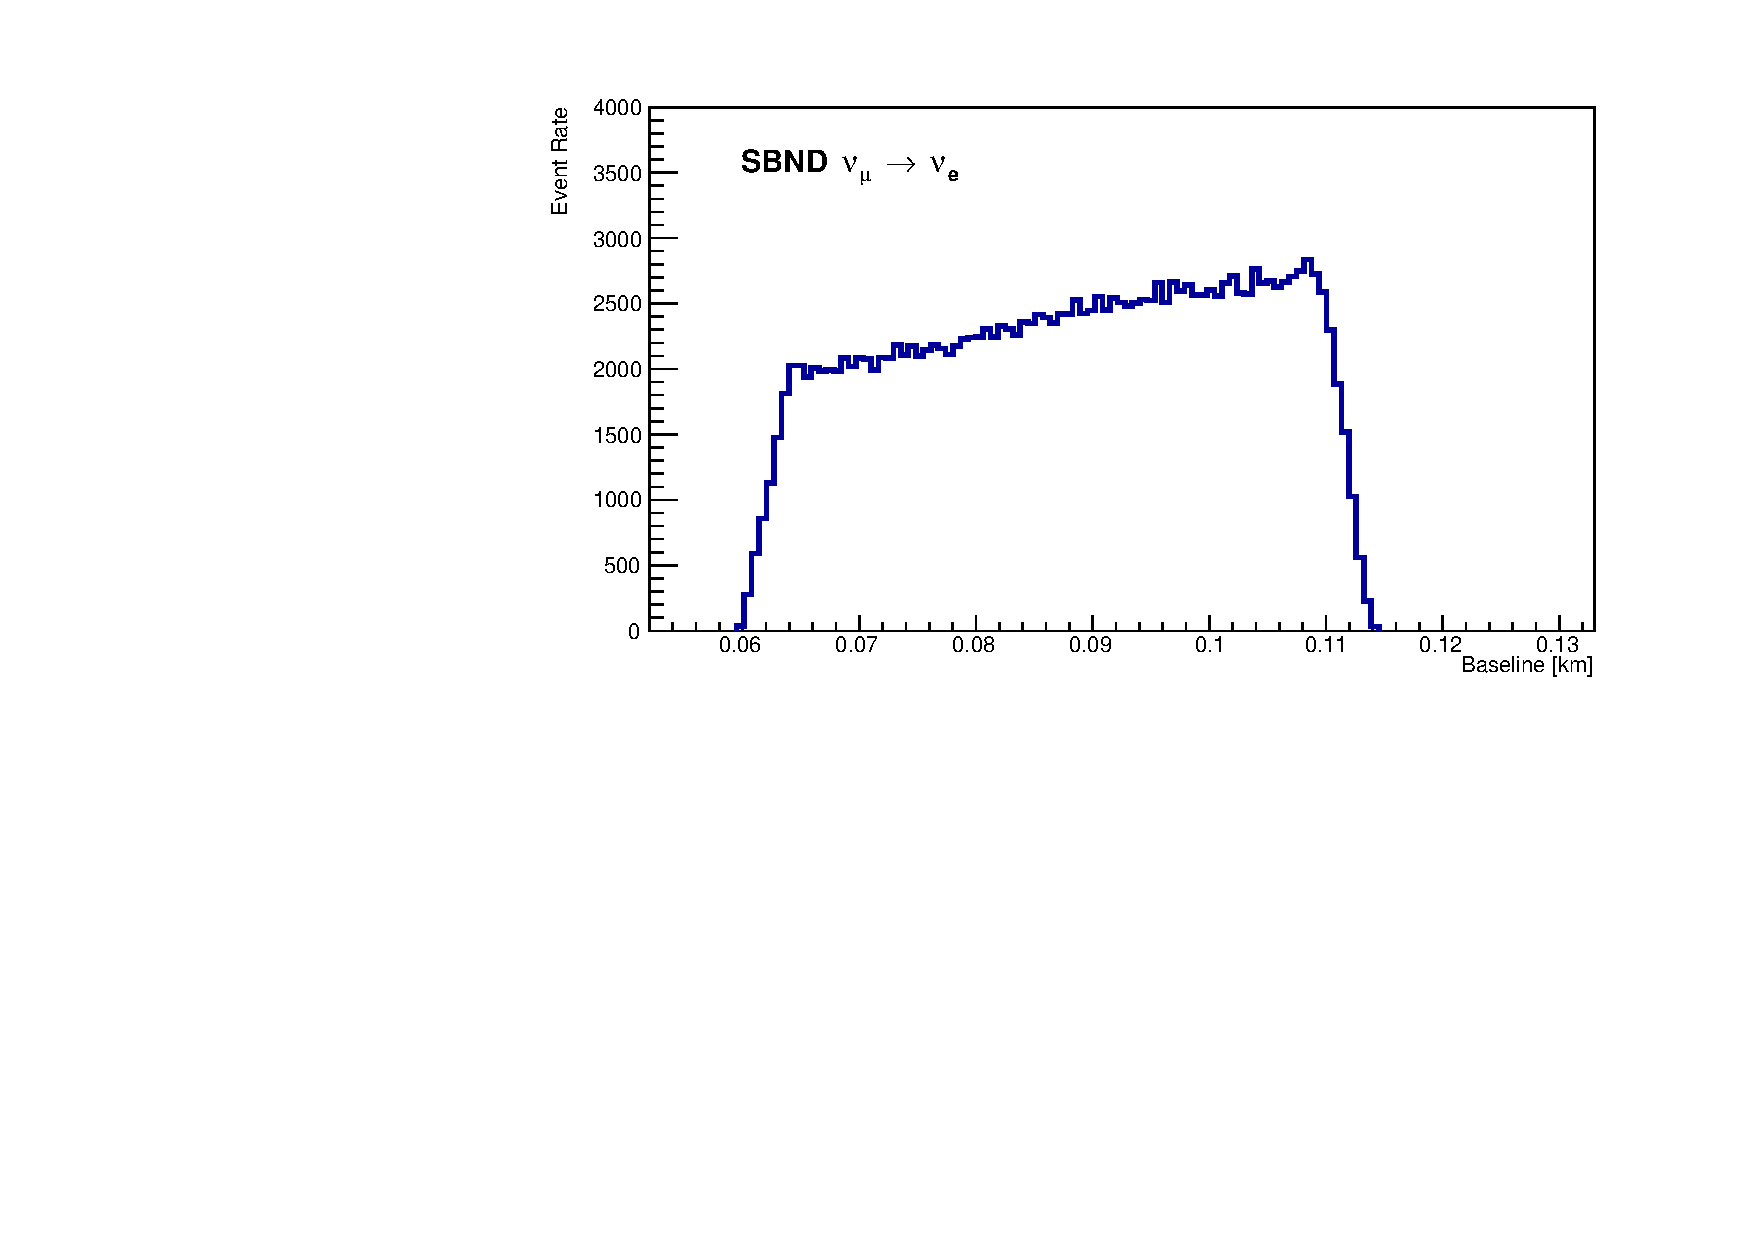
\includegraphics[width = 0.49\textwidth]{figures-chap5/SBND_osc.pdf}
    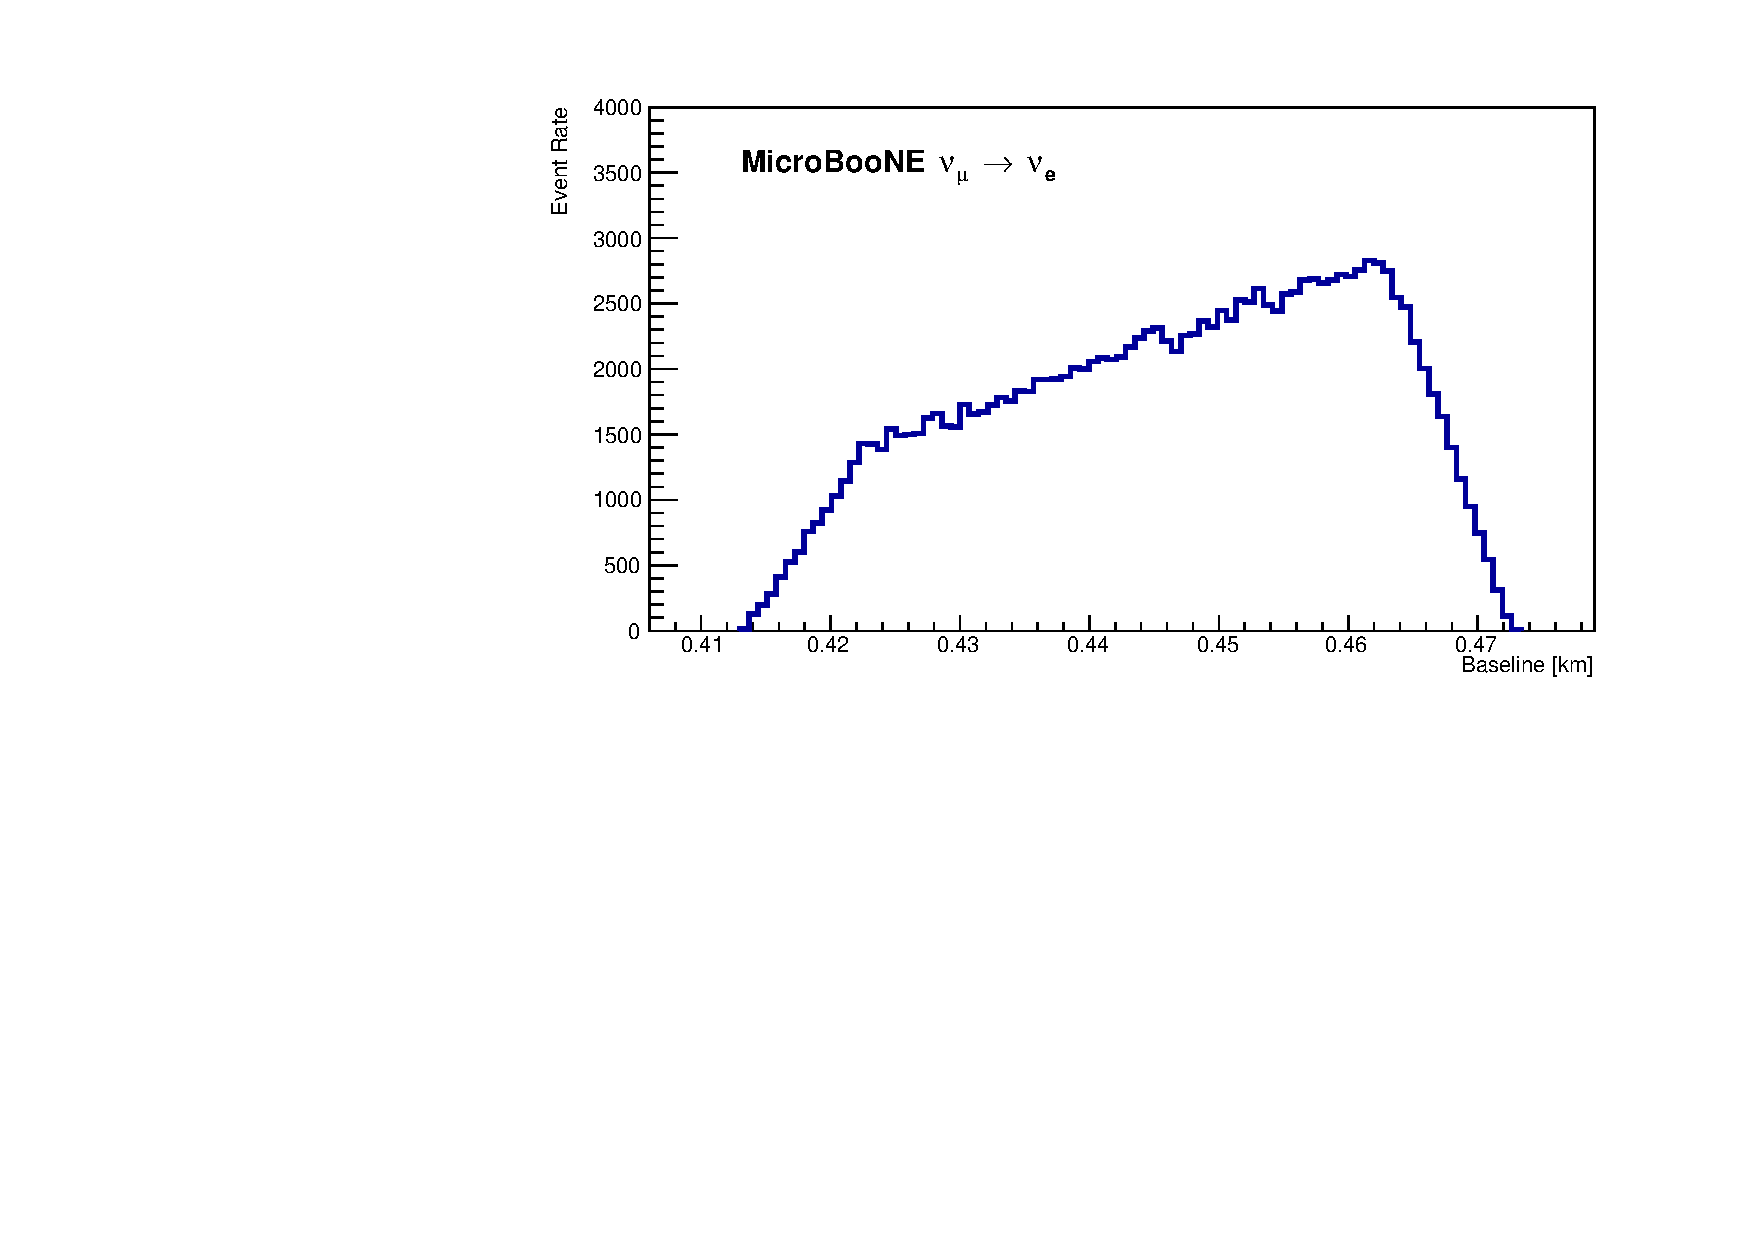
\includegraphics[width = 0.49\textwidth]{figures-chap5/MicroBooNE_osc.pdf}
    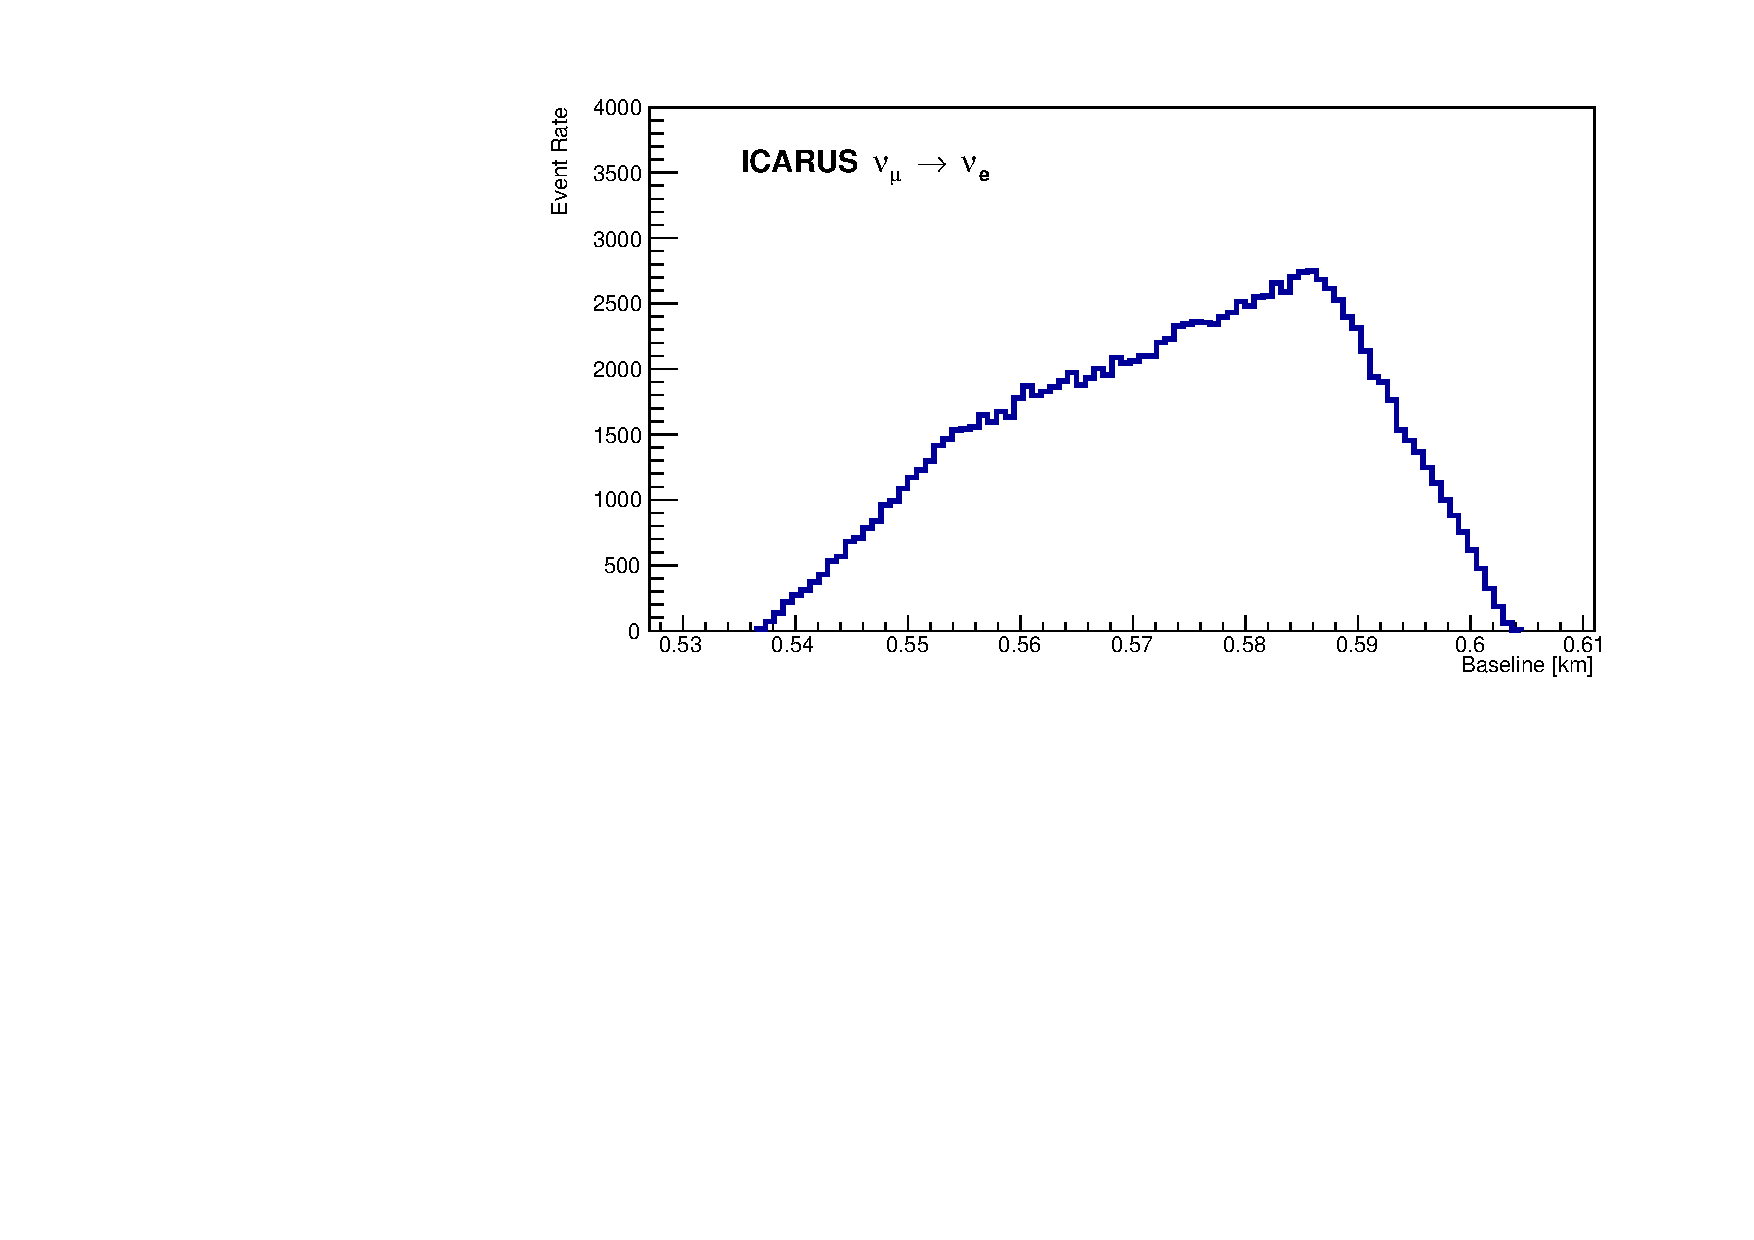
\includegraphics[width = 0.49\textwidth]{figures-chap5/ICARUS_osc.pdf}
    \captionsetup{width=0.45\textwidth}
    \parbox[b]{0.49\textwidth}%
    {
    \caption{The baseline distribution of events in the oscillated $\numu \rightarrow \nue$ sample for each of the \gls{sbn} detectors. \\\phantom{.}\\}
    \label{fig:nue_osc_baseline}
    }
  \end{figure}
  
  \begin{figure}
    \centering
    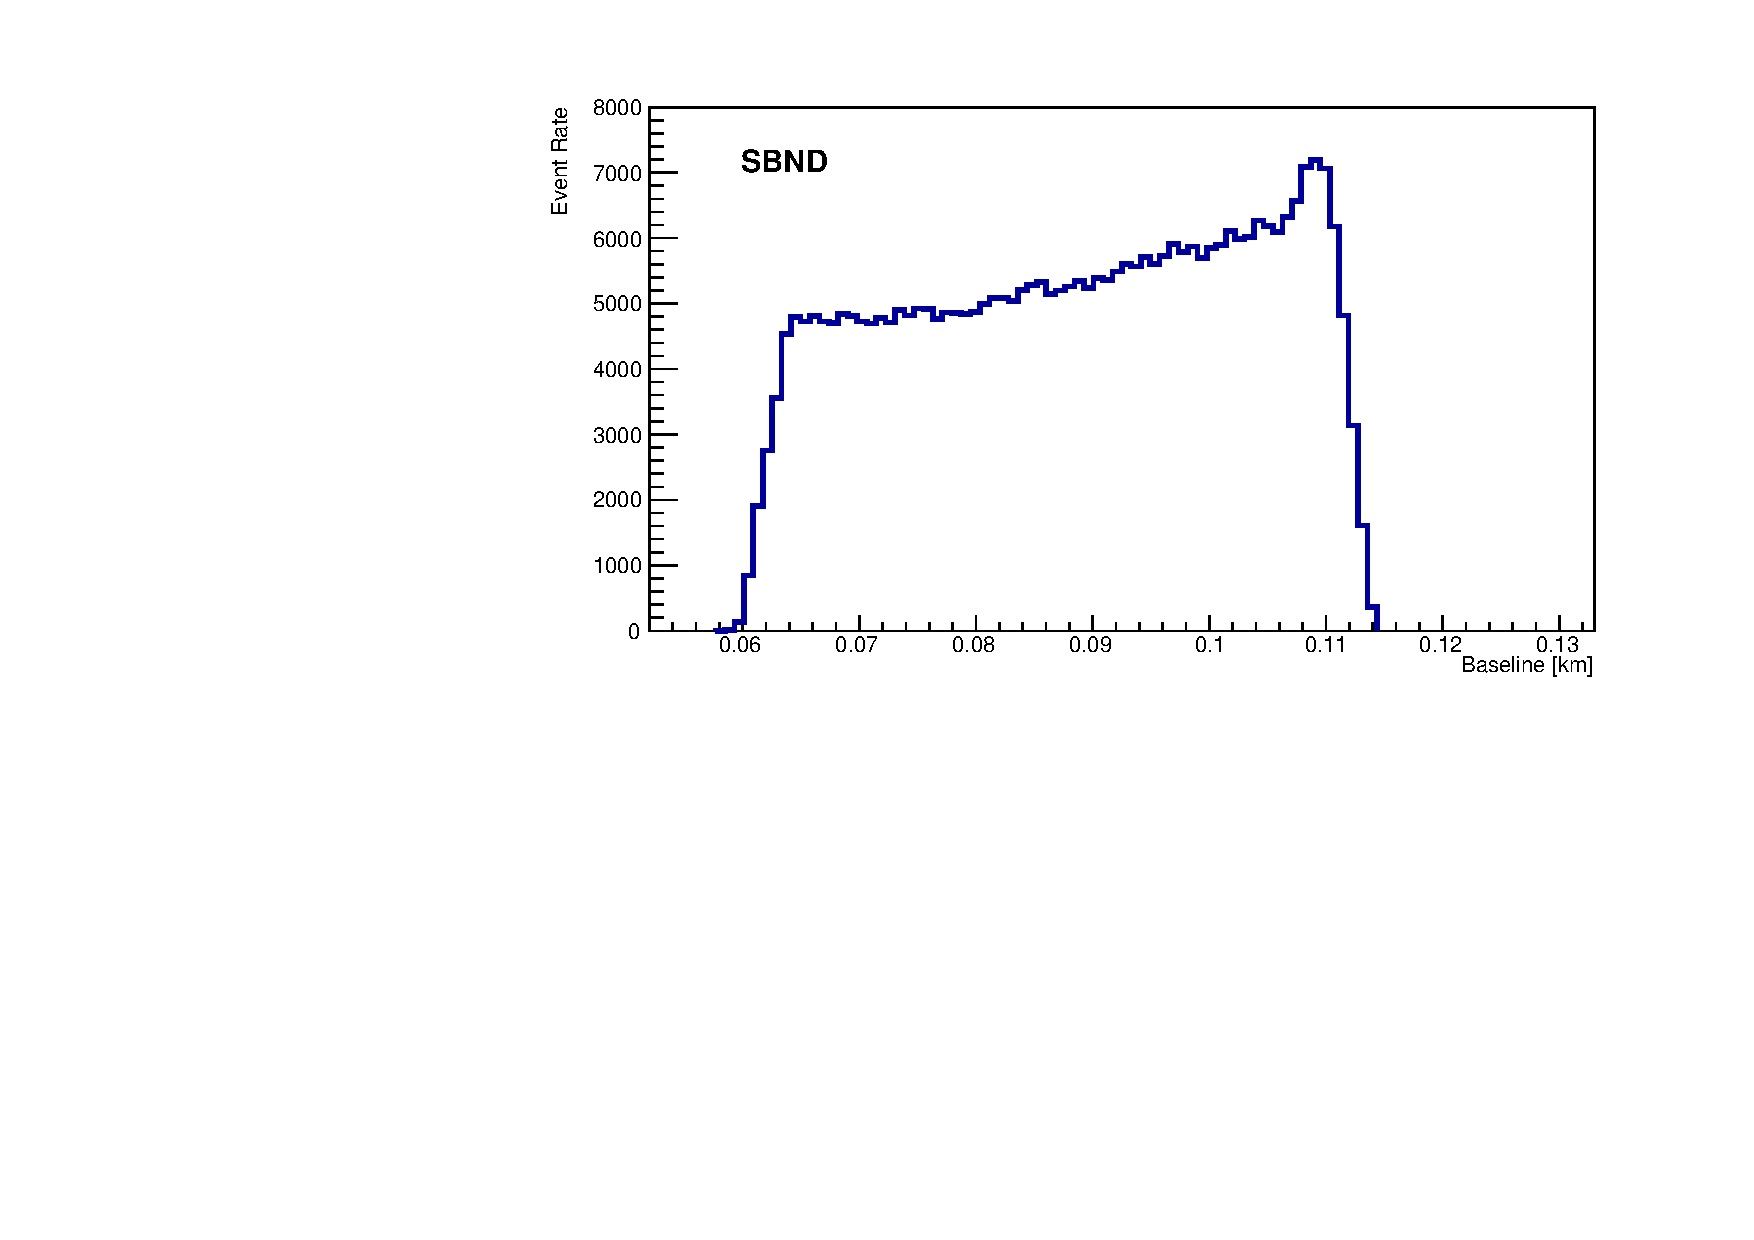
\includegraphics[width = 0.49\textwidth]{figures-chap5/SBND_nue.pdf}
    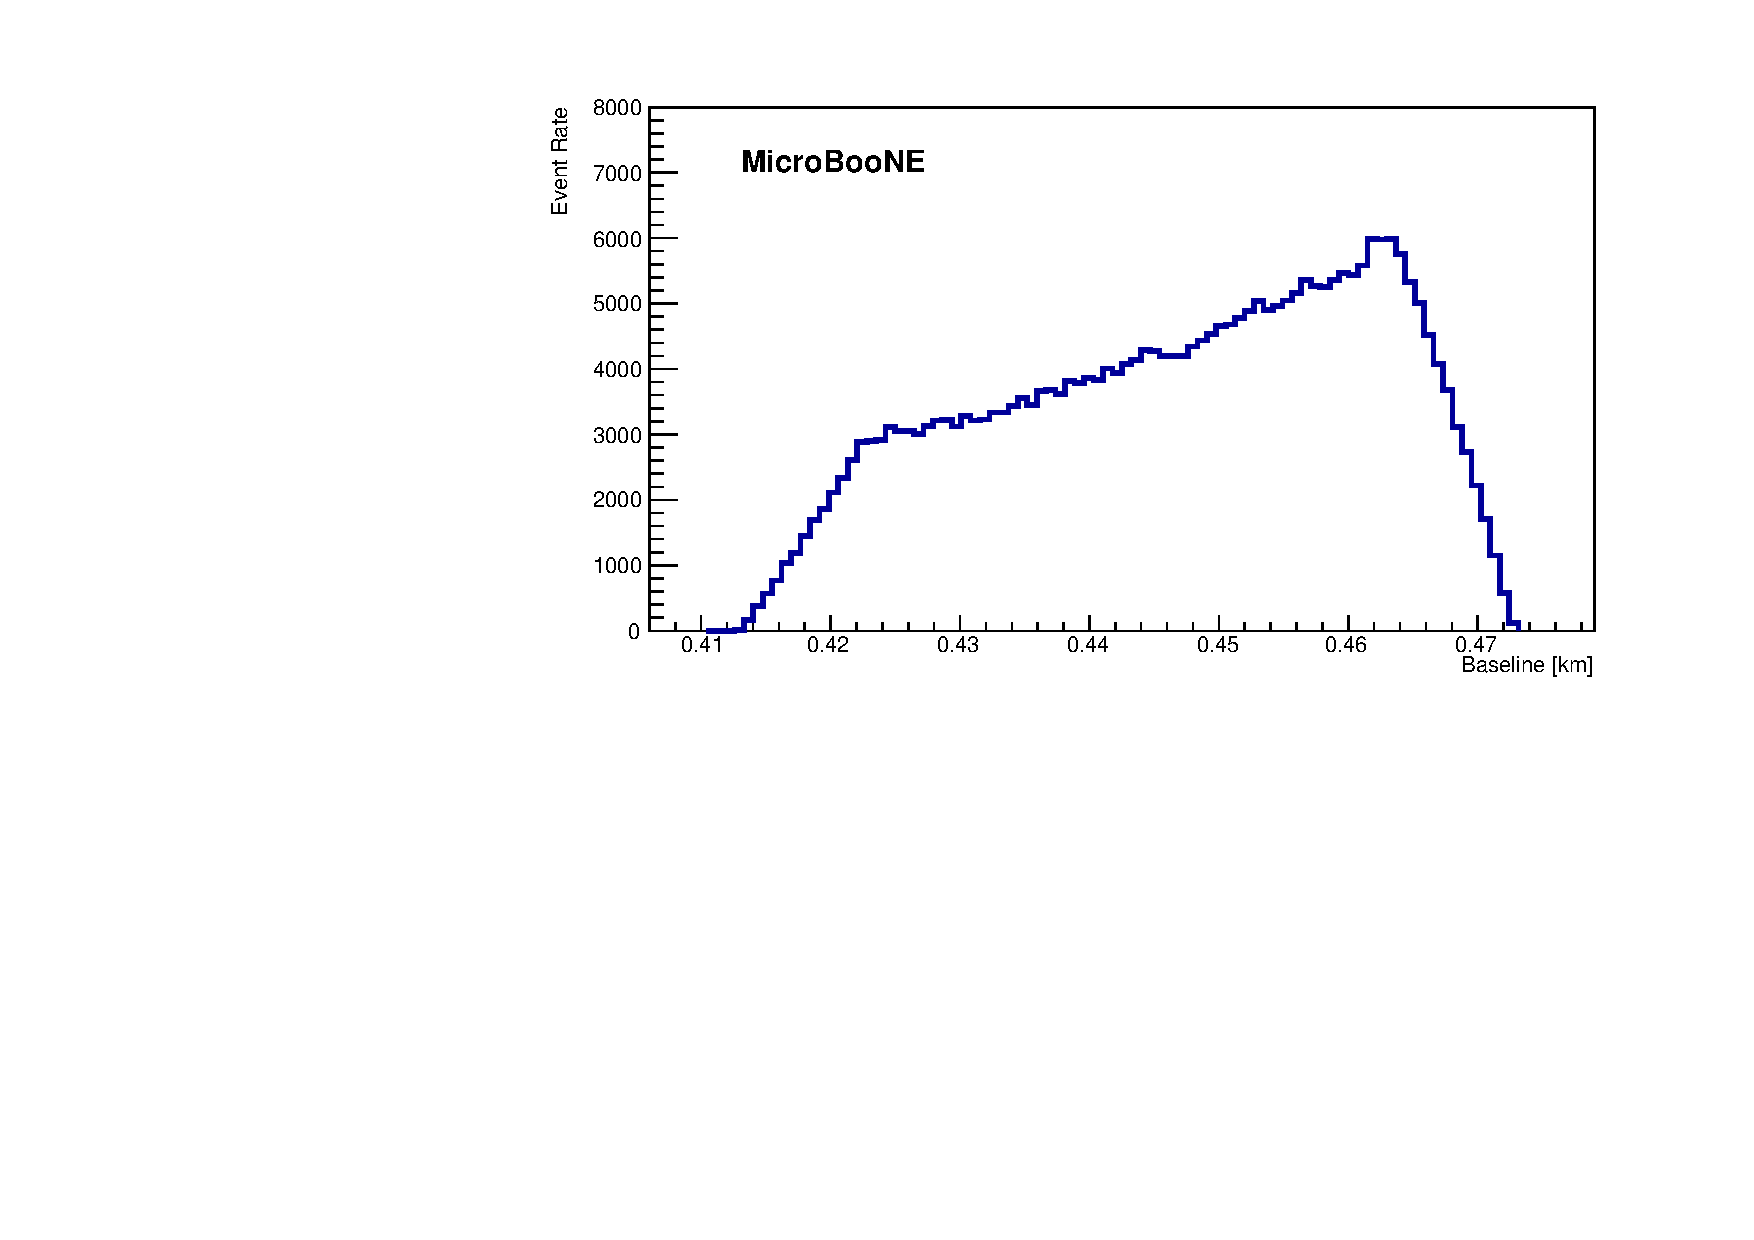
\includegraphics[width = 0.49\textwidth]{figures-chap5/MicroBooNE_nue.pdf}
    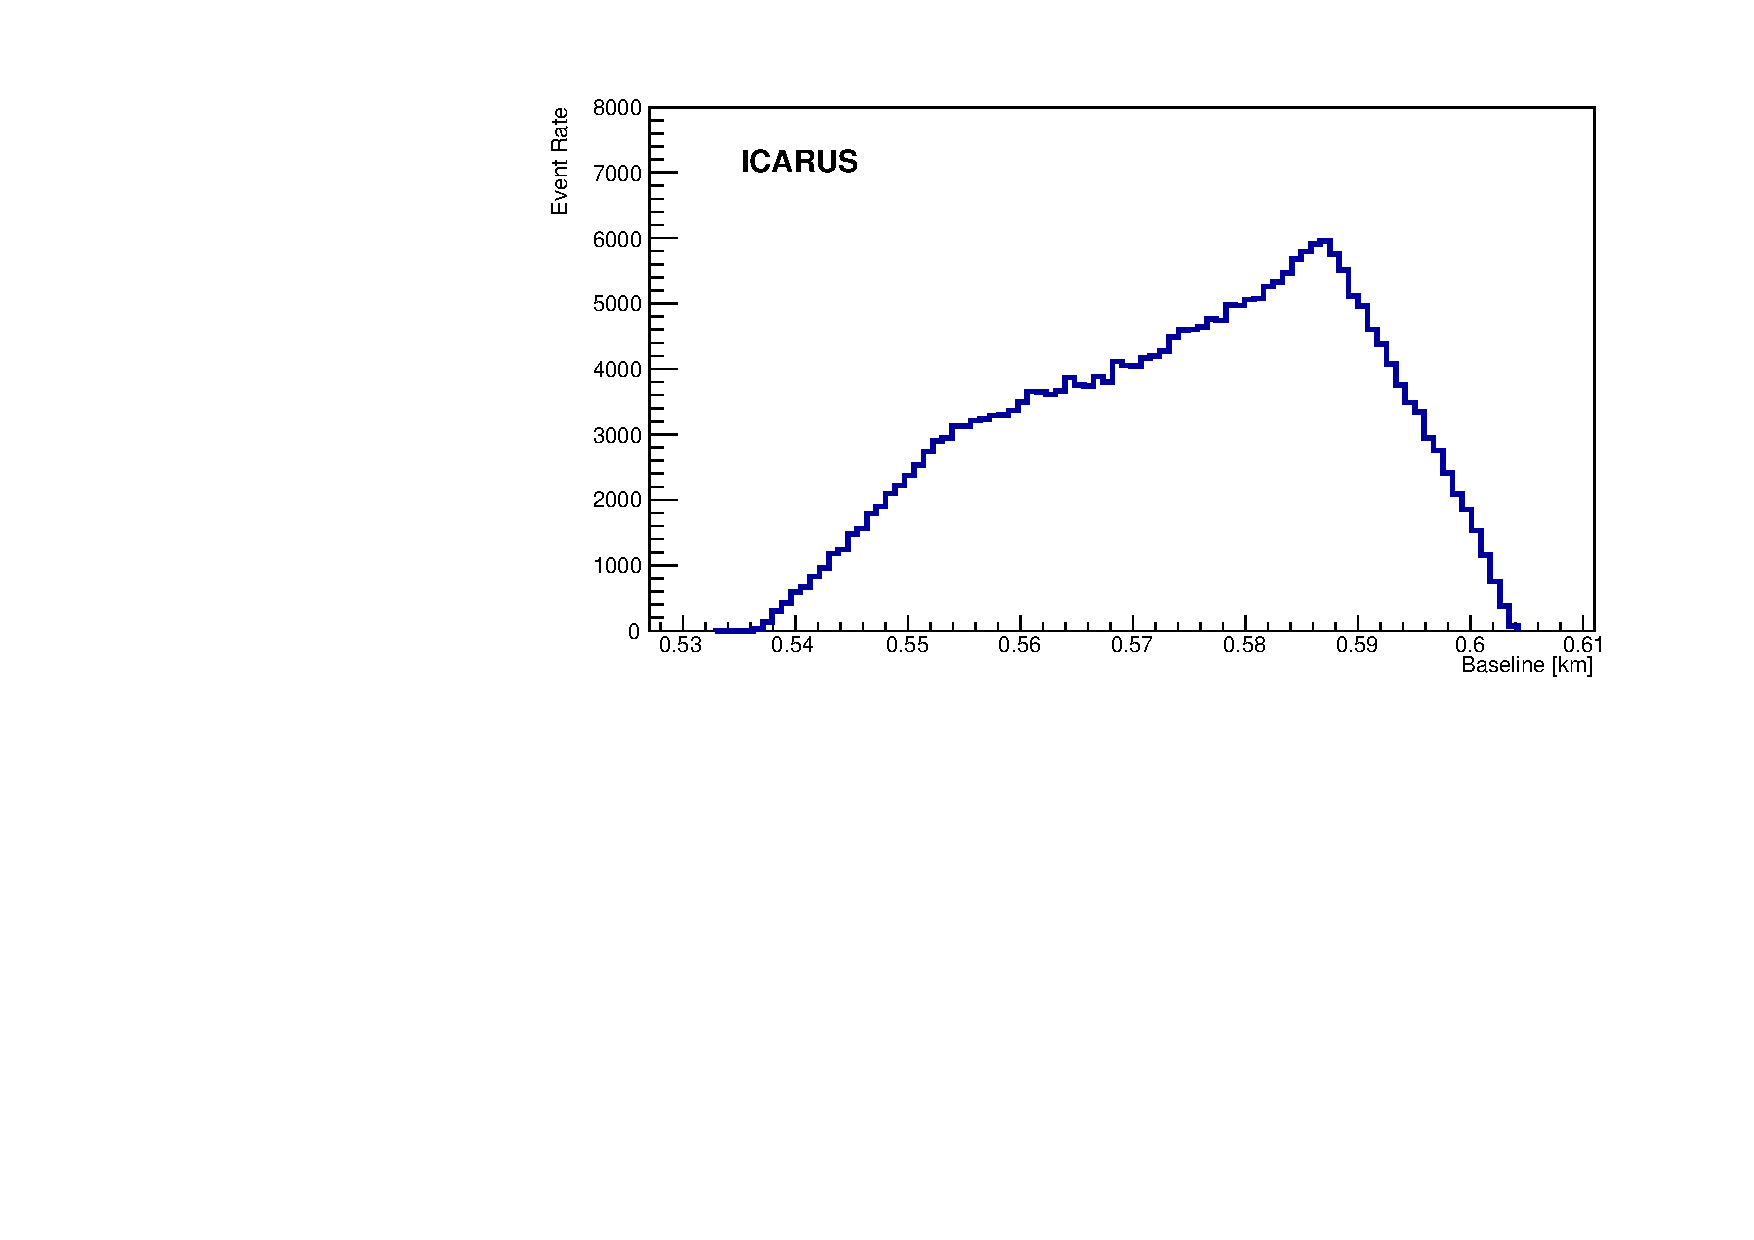
\includegraphics[width = 0.49\textwidth]{figures-chap5/ICARUS_nue.pdf}
    \captionsetup{width=0.45\textwidth}
    \parbox[b]{0.49\textwidth}%
    {
    \caption[The overall \nue baseline distributions.]{The baseline distribution of events in the overall \nue sample which is comprised of events from the intrinsic \nue, oscillated $\nu$, the \numu events from passing the \nue selection and the dirt and cosmic samples (which are not explicitly shown) for each of the \gls{sbn} detectors.}
    \label{fig:nue_baseline}
    }
\end{figure}

\begin{figure}[!h]
    \centering
    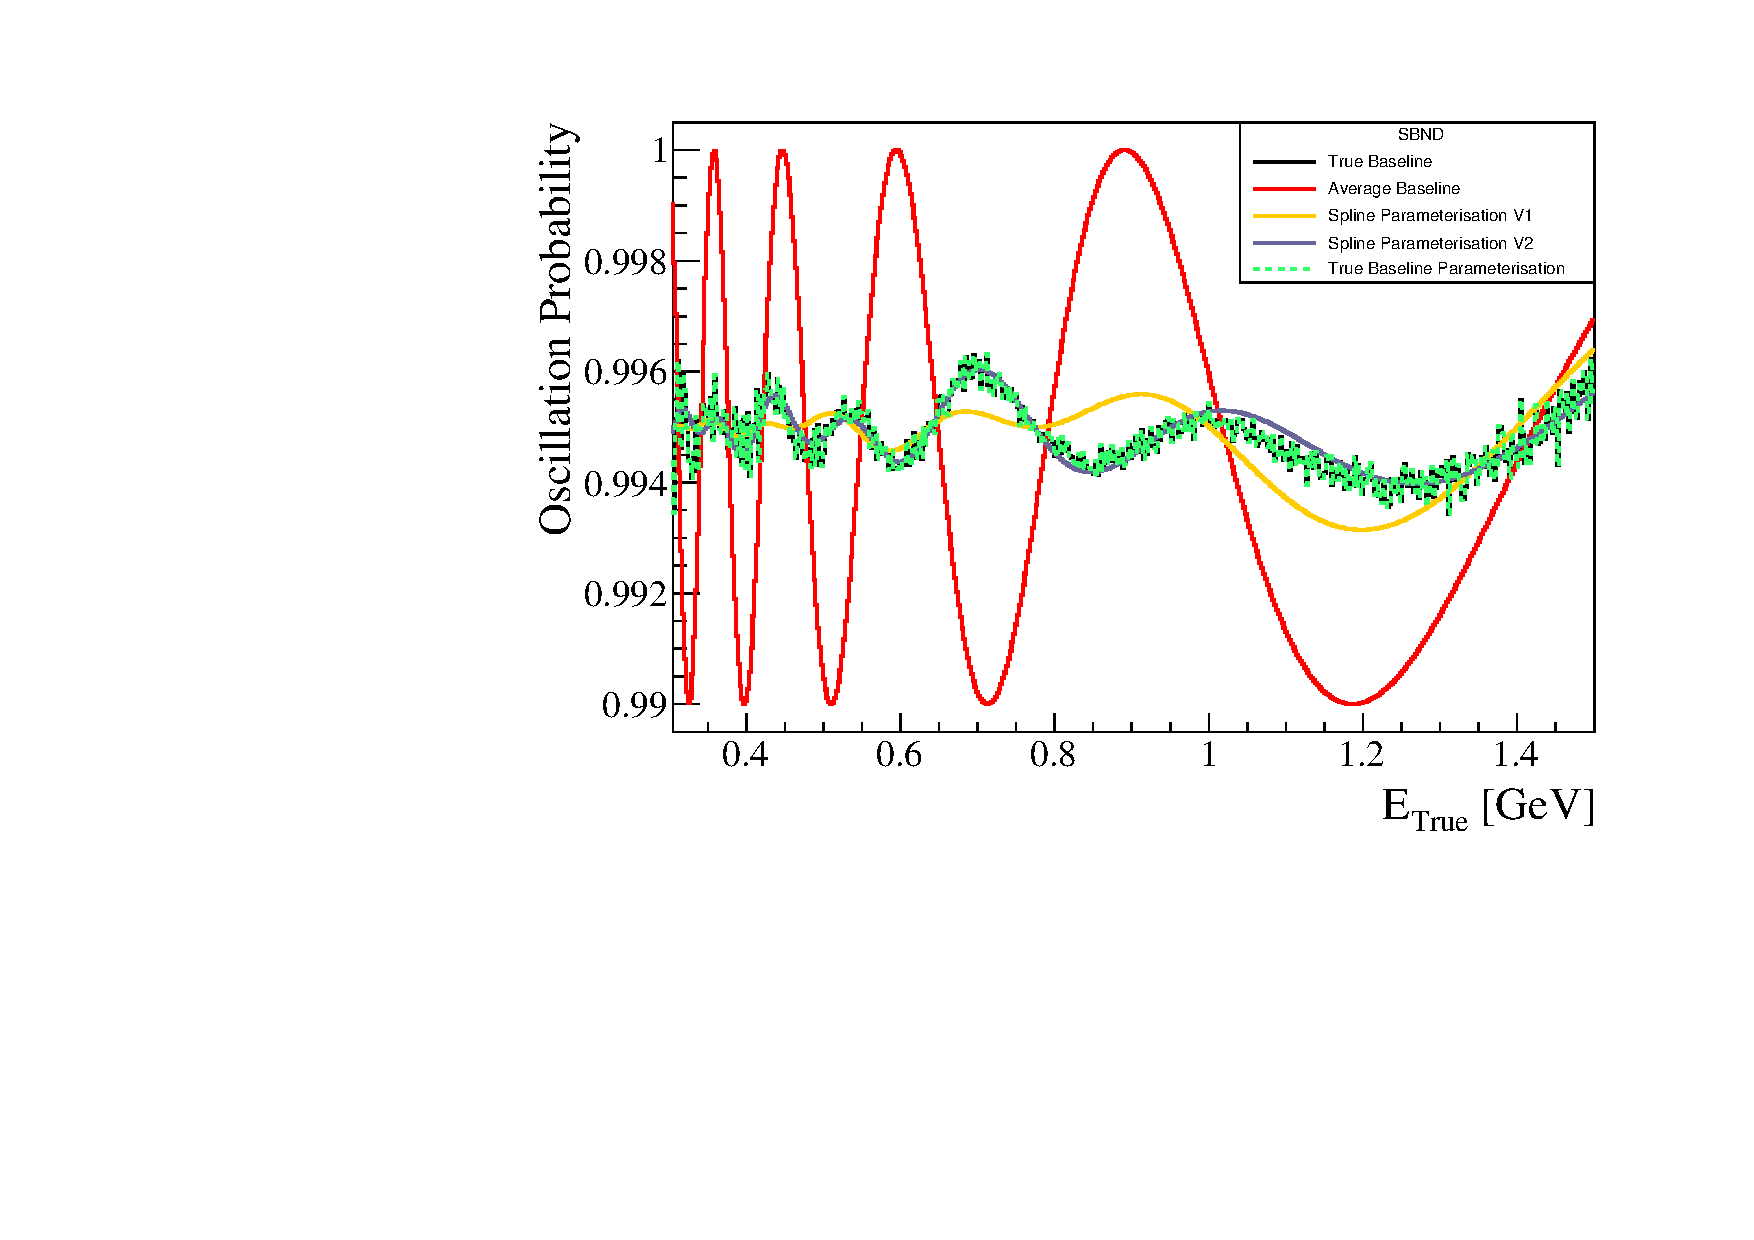
\includegraphics[width = 0.49\textwidth]{figures-chap5/osc_prob_sbnd.pdf}
    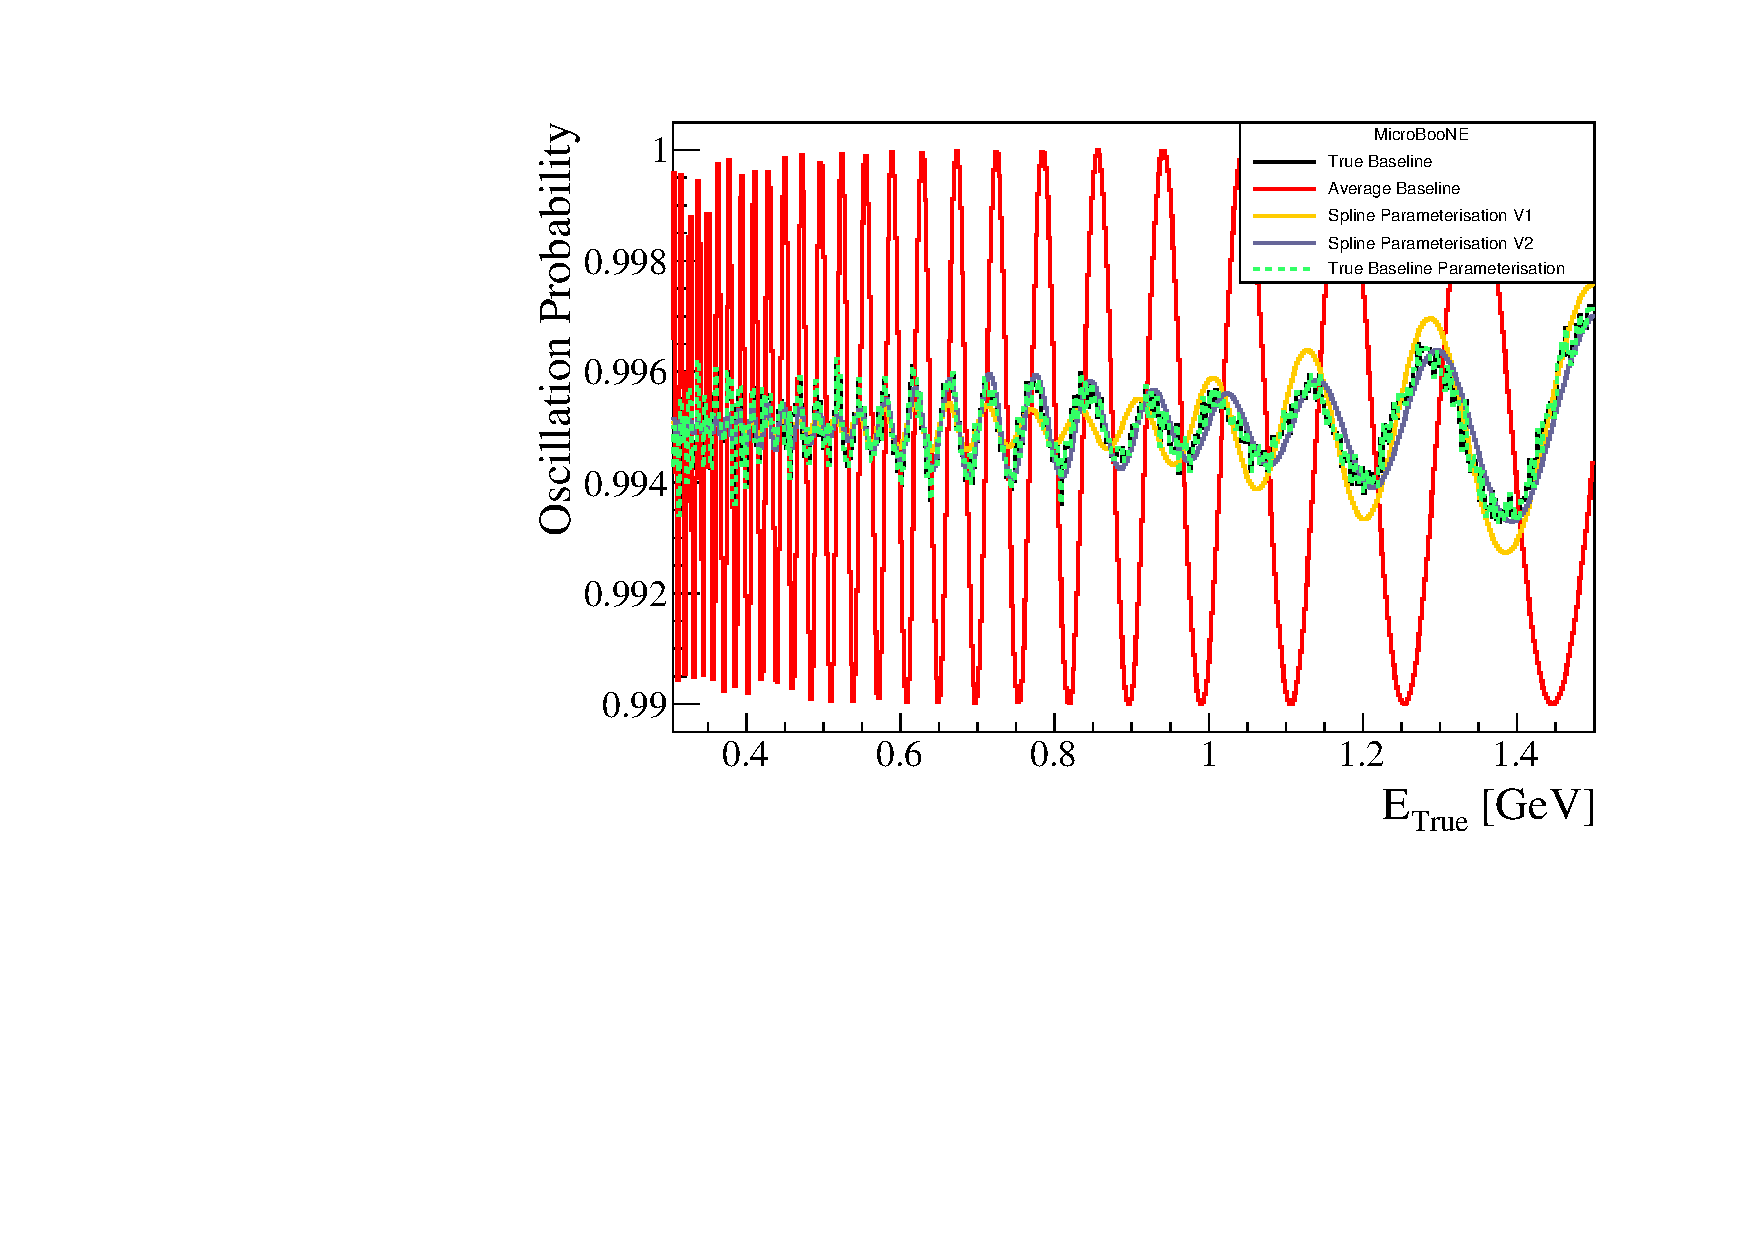
\includegraphics[width = 0.49\textwidth]{figures-chap5/osc_prob_uboone.pdf}
    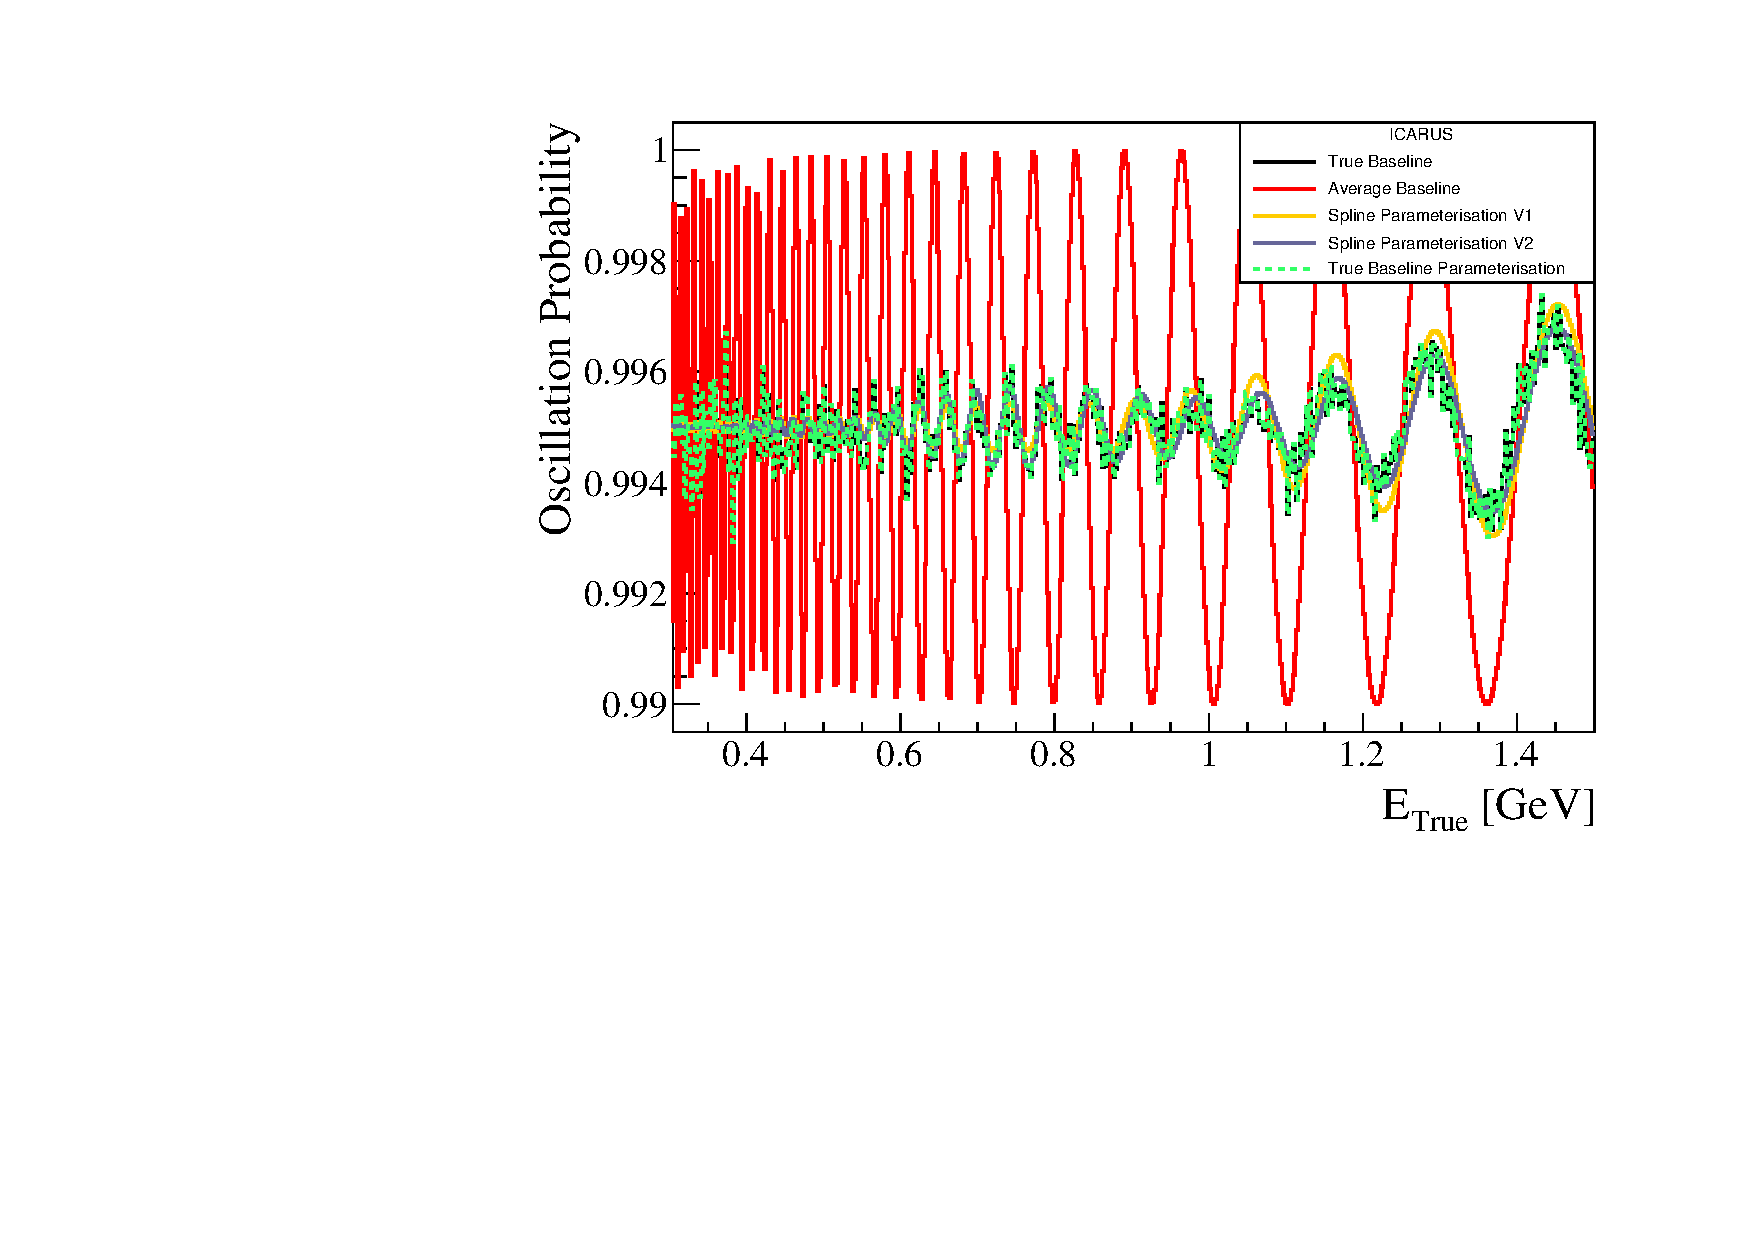
\includegraphics[width = 0.49\textwidth]{figures-chap5/osc_prob_icarus.pdf}
    \captionsetup{width=0.45\textwidth}
    \parbox[b]{0.49\textwidth}%
    {
    \caption[Oscillation probability for different baseline parametrisations.]{The oscillation probability as a function of true neutrino energy for the \numu disappearance sample with oscillation parameters $\sin^2{2\theta_{\mu\mu}} = 0.01$ and $\Delta m^2_{41} = 50$ eV$^2$ in each \gls{sbn} detector. The results from using each baseline parametrisation are shown. \\}
    \label{fig:baseline_osc_probability}}
\end{figure}

\clearpage
\subsection{Binning}\label{sec:binning}
The energy binning schemes used are the same across each of the three detectors, however, the scheme used is different for the \numu and \nue analyses. Furthermore, there are separate schemes for both the true and reconstructed energies. Each of the binning schemes is outlined below. 

The \numu edge-to-edge binning has 21 bins in reconstructed neutrino energy which are bounded as follows:
\begin{itemize}
    \item 1 bin from 0.00-0.20 GeV,
    \item 2 0.10-GeV bins from 0.20-0.40 GeV,
    \item 12 0.05-GeV bins from 0.40-1.00 GeV,
    \item 2 0.25-GeV bins from 1.00-1.50 GeV,
    \item 3 0.50-GeV bins from 1.50-3.00 GeV and
    \item 1 bin from 3.00-10.00 GeV.
\end{itemize}

The \numu edge-to-edge binning has 22 bins in true neutrino energy which are bounded as follows:
\begin{itemize}
    \item 1 bin from 0.00-0.30 GeV,
    \item 3 0.10-GeV bins from 0.30-0.60 GeV,
    \item 12 0.05-GeV bins from 0.60-1.20 GeV,
    \item 1 bin from 1.20-1.50 GeV,
    \item 3 0.50-GeV bins from 1.50-3.00 GeV,
    \item 1 bin from 3.00-5.00 GeV and
    \item 1 bin from 5.00-10.00 GeV.
\end{itemize}

The \nue edge-to-edge binning has 12 bins in reconstructed neutrino energy which are bounded as follows:
\begin{itemize}
    \item 1 0.35-GeV bin from 0.00-0.35 GeV,
    \item 5 0.15-GeV bins from 0.35-1.10 GeV,
    \item 2 0.20-GeV bins from 1.10-1.50 GeV,
    \item 2 0.25-GeV bins from 1.50-2.00 GeV,
    \item 1 bin from 2.00-3.00 GeV and
    \item 1 bin from 3.00-10.00 GeV.
\end{itemize}

The \nue edge-to-edge binning has 33 bins in true neutrino energy which are bounded as follows:
\begin{itemize}
    \item 2 0.25-GeV bin from 0.00-0.50 GeV,
    \item 15 0.05-GeV bins from 0.50-1.25 GeV,
    \item 15 0.25-GeV bins from 1.25-5.00 GeV and
    \item 1 bin from 5.00-10.00 GeV.
\end{itemize}

